%%
%%  This is a LaTeX template for an astronomy Bachelor's thesis.
%%
%%  Version 1.0
%%
%%  Authors: Anders Johansen, Sofia Feltzing, Johan Bijnens (2014)
%%  Send feedback to Anders Johansen <anders@astro.lu.se>
%%
\documentclass[12pt]{report}

\usepackage{a4wide}
\usepackage{graphicx}
\usepackage{natbib}
\usepackage[T1]{fontenc}  
\usepackage[utf8]{inputenc} 
\usepackage{geometry}
\usepackage[justification=centering]{caption}
\usepackage{subcaption}

\usepackage{fancyhdr}
\usepackage{lastpage}
\usepackage{pdfpages}
\usepackage{url}
\usepackage{listings}
\usepackage{color}

\pagestyle{fancy}
%\rhead{}
%\chead{}
%\lhead{}
%\rfoot{}
\cfoot{\thepage}
%\lfoot{}

\newcommand{\apj}{ApJ}
\newcommand{\apjs}{ApJS}
\newcommand{\apjl}{ApJ}
\newcommand{\mnras}{MNRAS}
\newcommand{\aap}{A\&A}
\newcommand{\aj}{AJ}
\newcommand{\nat}{Nature}
\newcommand{\pre}{Phys.~Rev.~E}
\newcommand{\araa}{ARA\&A}
\newcommand{\icarus}{Icarus}
\newcommand{\procspie}{Proceedings of the SPIE}




\definecolor{dkgreen}{rgb}{0,0.6,0}
\definecolor{gray}{rgb}{0.5,0.5,0.5}
\definecolor{mauve}{rgb}{0.58,0,0.82}

\lstset{frame=tb,
  language=Java,
  aboveskip=3mm,
  belowskip=3mm,
  showstringspaces=false,
  columns=flexible,
  basicstyle={\small\ttfamily},
  numbers=none,
  numberstyle=\tiny\color{gray},
  keywordstyle=\color{blue},
  commentstyle=\color{dkgreen},
  stringstyle=\color{mauve},
  breaklines=true,
  breakatwhitespace=true,
  tabsize=3
}

\begin{document}

\title{\huge \bf Multi-planetary Systems from Simulated TESS Transit Timing Variations\footnote{This is just a very basic cover page produced by LaTeX -- when
the thesis is done you can get a more formal cover page from Eva Jurlander.}}
\author{Lucas Hellström}

\thispagestyle{empty} % do not count pages just yet

\maketitle

\newpage

\thispagestyle{empty}

\begin{center}
  (this page will contain some more official information in the final version)
\end{center}

\newpage

\thispagestyle{empty}

\begin{center}
  {\bf Abstract}
\end{center}
	A transit is a phenomenon where a planet passes between its host star and an observer blocking out part of the light from the star. This decrease can be measured and used to gain information about the planet. The Kepler and TESS telescopes are examples of space telescopes using the transit method to detect exoplanets. For systems with more than one planet around the same star variations between the time a planet takes to transit might occur. These variations, called Transit Timing Variations, or TTVs, can be used to gain information about additional planets in the system.
	
	TESS recently launched and this paper uses data from \cite{2015ApJ...809...77S} and Kepler data from Q1-Q17 DR25 from the NASA Exoplanet Archive (Thompson et al. 2018) to create artificial systems like those that TESS might observe to predict what kind of results it might find. These systems are simulated using TTVFast \citep{2014ApJ...787..132D} to obtain TTV signals which are then used to create a sky map to show the fraction of systems showing TTV signals in a given sample.
	
	TESS have coverage of the ecliptic poles for a whole year which results in that many systems showing considerable TTV signals being located at the poles although there are systems located outside the poles still showing TTV signals. In the range of declination from about $-40^{\circ}$ to $40^{\circ}$ CHEOPS will be able to further study the objects. As CHEOPS will study already known objects predictions for the results from TESS can be used to estimate the number of targets CHEOPS might study, how much observation time is required for each object and how to prioritise the most interesting systems. Using information about the planetary radius, period and stellar mass obtained from short-term observations the long term TTV amplitude can be estimated. From the results of this paper it is expected that CHEOPS can find a TTV signal from about every fourth transiting planet and the probability for a CHEOPS detectable TTV signal is high where the period ratio is below 2 but low for a higher fraction.
	
	
\newpage

\thispagestyle{empty}
\mbox{} % this is how we create an empty page in LaTeX

\newpage

\thispagestyle{empty}

\begin{center}
  {\bf Popul\"arvetenskaplig beskrivning}
\end{center}
	När vi letar efter exoplaneter finns det ett antal olika metoder för att hitta dem. Den mest framgångsrika är transitmetoden där ljusstyrkan hos en stjärna studeras under en längre tid. När en planet passerar mellan sin stjärna och en observatör kan en minsking i stjärnans ljusstyrka ses. Uppreras detta i regelbunda intervall kan slutsatsen att det finns en planet runt stjärnan dras. Genom att studera minskningen i ljusstyrka kan storleken på planeten beräknas vilket kombinerat med massan som fås av andra metoder ge en insikt i hur och vad planeten är uppbygd av. En transit är detta fenomen då en planet passerar mellan stjärnan och en observatör.
	
	Genom att jämföra tiden mellan varje transit för en planet kan ibland variationer ses, vilket kallas Transit Timing Variations eller förkortat TTV. Detta beror på att det finns fler planeter runt stjärnan som med hjälp av gravitationskraften accelererar eller decelerera planeten som bevakas. Detta resulterar i att det är möjligt att hitta planeter som genom andra metoder är osynliga. 
	
	Keplerteleskopet är ett rymdbaserat teleskop som använder transitmetoden för att hitta exoplaneter. Det har sedan 2009 hittat över 1000 bekräftade exoplaneter vilket gör den till det hittils mest framgångsfulla uppdraget i jakten på exoplaneter. TESS, vilket står för Transiting-Exoplanet Survey Satellite, är ett teleskop som sköts upp den 18de april 2018 och använder transitmetoden för att hitta exoplaneter. TESS kommer bli det första rymdbaserade teleskopet att studera hela himlen och kommer observera över 200 000 stjärnor under uppdragets urspungliga längd på två år.
	
	Detta projekt kommer använda data från Keplerteleskopet för att simulera data från TESS för att sedan använda den datan för att leta efter TTV signaler. Detta ska ge en uppfattning om hur många system som har fler än en planet inom ett givet område på himlen.
	
	


\newpage

\thispagestyle{empty}
\mbox{} % make sure that TOC starts on a right page

\newpage

\setcounter{page}{1} % start counting pages

\tableofcontents

\newpage

\listoffigures 
%\listoftables

\newpage

\chapter{Introduction}
When observing stars in the search for exoplanets a few different methods can be used. The most successful method so far is the transit method which measures the brightness of a star for a long period. If a planet passes between the star and the observer it will block out part of the light and the brightness will decrease. If these decreases occur at regular intervals the conclusion that the reason for this is an exoplanet can be drawn. By studying the amount of light the planet blocks out the radius of the planet can be found; combined with the mass of the planet obtained from different methods the approximate density of the planet can be calculated. This gives information about the structure and composition of the planet.

In a system with multiple planets around the same star, the plants will affect each other through their gravitational pull. This results in the planets accelerating or decelerating depending on the relative positions of the planets. As this is happening the time of one orbit may differ and by studying these variations, planets which may not be possible to detect through the transit method can be detected \citep{2012Sci...336.1133N}. TTVs can also be used to calculate the mass of the transiting planet and is commonly used to confirm exoplanet candidates as real planets.

This paper will simulate data from the TESS telescope to search for these transit timing variations in order to determine the approximate fraction of multi-planetary systems in a given sample. The amplitude dependence on observation time is plotted and compared to a analytically approximation to understand the importance of longer observation times in order to detect TTVs. Finally systems in the range where CHEOPS are able to observe will further be studied in order to determine the fraction of detectable TTV signals based on the radius and period ratio of the planets in the system which will predict what kind of systems are best suited for follow-up observations.

\section{Transits}
	A planet in orbit around its host star may sometimes cross the line of sight of an observer. When this happens a slight decrease in the star's brightness can be measured. This is called a transit and is today used as a main method to discover exoplanets. From transits the radius of the planet can be determined but it can also be used to find additional planets around the host star which may not be transiting. This will be discussed in section \ref{sec:trans_vari}. With the radius known from the transit method and the mass obtained from for example the TTV signal or different methods such as, for example the radial velocity method, the density of the planet can be calculated. The density is important to understand what the planet is made of and the structure of it.

\subsection{Variations}
\label{sec:trans_vari}

	For a system with a single planet around a star the period of the planet is more or less perfectly periodic with no visible variations but, when measuring the time of between a planet's transits one may discover variations in the period which are called Transit-Timing Variations or TTVs. These variations arise from another planet in the system whose gravitational pull accelerates or decelerates the observed planet which results in increased or decreased transit times. The amplitude of the TTV signal is dependent on the mass of the planets and the ratio of the periods between them, some rations give rise to a resonance which increases the amplitude of the TTV \citep{0004-637X-688-1-636}. TTV signals are typically sinusoidal \citep{2012ApJ...761..122L} with a period called the super-period. This super-period is heavily dependent on resonance of the period fraction and are often in the range of 10 to 100 days. This means that the period of many TTV signals are too long to be observed by a single TESS observation period and requires further measurement. An advantage of studying transits in search for TTVs is that planets which does not transit their star can be discovered through TTVs \citep{0004-637X-777-1-3}. As most planets does not transit their star this can increase the number of known exoplanets drastically.

\section{Kepler}
	The Kepler satellite launched in spring 2009 on a mission to study stars in a small patch in the sky to discover Earth-sized exoplanets within the habitable zone, where liquid water can exist on the planetary surface. The brightness of a large amount of stars are measured and then analyzed in order to detect transiting exoplanets. 
	
	Kepler started by looking at a very small patch of the sky but in July 2012 one of the four wheels used to keep the patch in focus broke. The telescope requires at least three wheels to function which kept the mission alive. In May 2013 a third wheel failed which resulted in the telescope no longer being able to collect data. The satellite was nonfunctional until the so-called "Second Light (K2)" in early 2014. This mission would use the telescopes remaining two wheels to study stars over a much larger area but for shorter periods. \citep{2017PAPhS.161...38B}
	
	Kepler have found over 4500 exoplanet candidates \citep{2017PAPhS.161...38B} to this day. This amount makes Kepler the most successful exoplanet hunting mission to this date.
	
	
\section{TESS}
	The Transiting Exoplanet Survey Satellite, TESS, is a satellite which were launched on the 18th of April 2018. The satellite is equipped with four cameras which will study the brightness of over 200 000 stars over a two year period. It is the first all-sky transit survey taking place in space. \citep{2014SPIE.9143E..20R}
	
	TESS will study the whole sky by splitting it into 26 sectors, 13 in the southern hemisphere and 13 in the northern hemisphere, which are observed for 27 days each. An illustration of this can be seen in figure \ref{fig:tess_time} where the number of times TESS will observe each sector is shown. TESS will observe the southern hemisphere during the mission's first year, it will then rotate and observe the norther hemisphere for another year.
	\begin{figure}[h!]
	\centering
		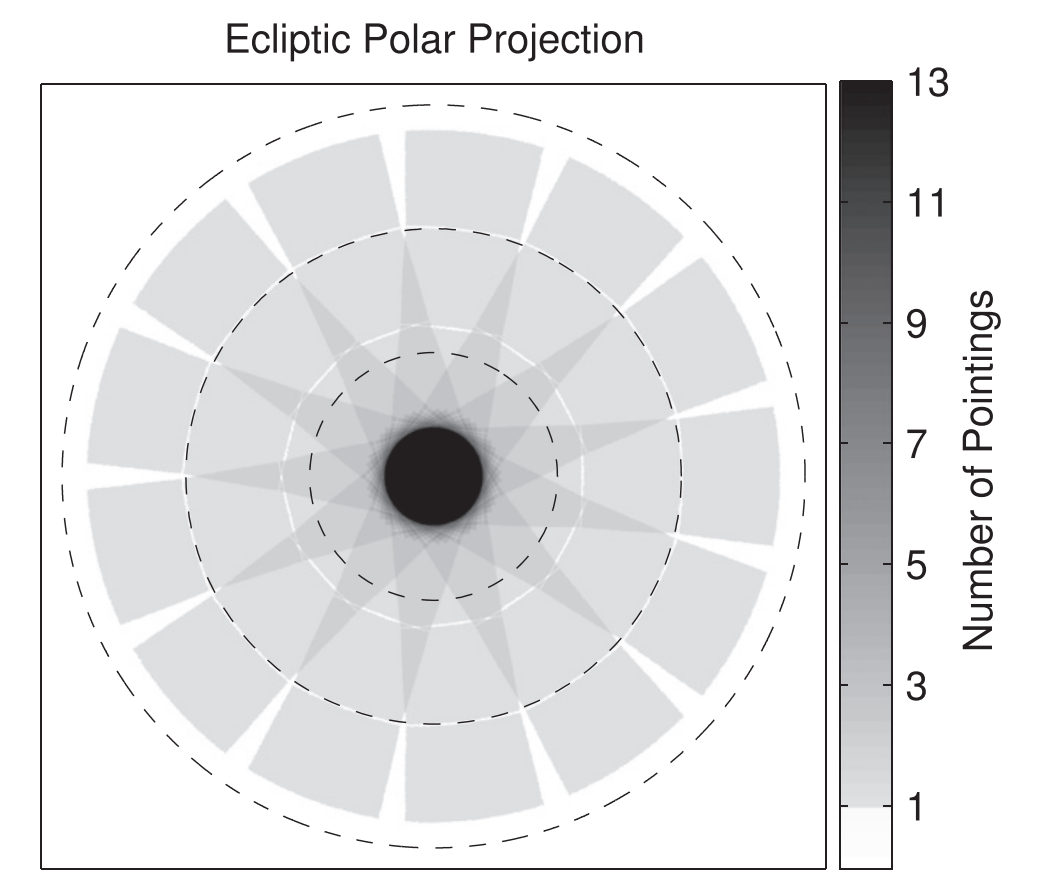
\includegraphics[width=0.8\textwidth]{img/tess_observe_time.png}
		\caption{Illustration of the number of times TESS will observe each sector in the sky.\\ \small{Source: \cite{2015ApJ...809...77S}, figure 1}}
		\label{fig:tess_time}
	\end{figure}	
	
\section{CHEOPS}
	The CHaracterising ExOPlanets Satellite, CHEOPS, is a satellite currently in development which is planned to launch in early 2019. It will study already known bright stars hosting planets for transits with ultrahigh precision photometry \citep{2013EPJWC..4703005B}. 
	
	TESS will discover several hundreds systems and give a fair estimation of the planetary radius and mass of transiting planets in these systems. TESS will also be able to find TTV signals for systems with a low super-period. CHEOPS will be able to use this data to look at planets with mass between $1\; M_{\oplus}$ and $20\; M_{\oplus}$ in order to obtain more accurate radii measurements which in turn can be used to determine the structure which might help in understanding the formation and evolution of planets in this mass range. CHEOPS will also be able to make follow-up TTV measurements for more accurate TTV data.
	
	Due to limitations on CHEOPS it is not able to study the whole sky and is limited to a range of about 40 degrees above and below the ecliptic. This creates a problem with candidates to observe obtained from TESS as the systems in this range are only observed for one or two observation periods while the ecliptic poles have all year coverage.
	
\chapter{Method}
	This paper uses results from \cite{2015ApJ...809...77S} where potential system which TESS might find are simulated. A limitation of the simulated detections by Sullivan et al. is that, although they report the number of planets per star, parameters for only one planet are actually provided. However, we can use the lare number of multi-planet systems discovered by Kepler to create artificial systems based on the results from Sullivan et al. and the Kepler dataset. These systems are then simulated to obtain TTVs. The steps taken are listed below:
	
\begin{enumerate}
	\item For each planet in the Sullivan et al. catalogue a similar planet within 10\% in radius and period are found in the Kepler dataset.
	\item The system are then filled with additional planets taken from the Kepler archive and modified based on the ratio of the radius and period of the first Sullivan and Kepler planet. The planetary period and signal-to-noise ratio for all planets are checked in order to ensure that they are detectable by TESS.
	\item These planets are then assigned a mass depending on the radius of the planet \citep{2015ApJ...809...77S} and an eccentricity based on a Rayleigh distribution as none of those parameters are obtained from the light curves.
	\item The systems are then simulated using TTVFast \citep{2014ApJ...787..132D} and the resulting transit times are analyzed. First a linear fit needs to be applied and subtracted to remove the period of the planet and thus obtain the variation. The amplitude of the variation is obtained from average of the highest and lowest value.
	\item The same procedure, mass-radius relation and  distribution are applied to Kepler systems and the results compared to the TTV catalogue of \cite{2018ApJS..234....9O} to verify that the methods and assumptions give realistic results.
	\item The error of the results are calculated from \cite{2005Sci...307.1288H} and is dependent on the magnitude of the host star, the ratio of radius between the planet and host star and the transit duration.
	\item To ensure that the systems are realistic they are simulated for stability over a long time. This is done using WHFast \citep{2015MNRAS.452..376R} and IAS15 \citep{2015MNRAS.446.1424R}.
	\item The amplitude dependence on observation time are plotted and compared to an analytical approximation, giving an idea of how the amplitude increases over time. This shows the importance of longer observation times in order to obtain full TTV signals.
	\item Systems in the CHEOPS observation range, $-40 < \beta < 40$, are further studied in order to obtain the fraction of planets showing a TESS detectable TTV signal for a given radius and period ratio.
\end{enumerate}

\section{Simulation of TESS objects}
\label{simTESS}
	\cite{2015ApJ...809...77S} provides one planet per system. By combining data from Kepler obtained from the Kepler dataset\footnote{\url{https://exoplanetarchive.ipac.caltech.edu/index.html}} and the results from Sullivan et al., we simulate artificial TESS systems to obtain TTV signals. Sullivan et al. uses the occurrence rates of planets around a host star with effective temperature $T_{eff} < 4000$ K from the results reported by \cite{2015ApJ...807...45D} while for $T_{eff} > 4000$ K the occurrence rates are obtained from \cite{2013ApJ...766...81F}. Because of this the planets are separated into two groups based on the effective temperature of the host star. One group with effective temperature below 4000 K and one for higher.

	For each planet in the Sullivan et al. catalogue, a similar planet, in radius and period, are selected from the Kepler dataset. This planets in this system are then verified that their period is not longer than the observation time of TESS and the Signal-to-Noise Ratio, SNR, of this system from the Kepler dataset is compared to a calculated SNR:
	\begin{equation}
	SNR = \frac{T_{depth}}{N_{6}}
	\end{equation}	
	where $T_{depth}$ is the transit depth and $N_{6}$ is the noise from 6 hours of observations:
	\begin{equation}
	SNR = \left(\frac{R_p}{R_{\star}}\right)^2 \times \sqrt{6\Gamma}
	\end{equation}
	where $R_p$ and $R_{\star}$ is the radius of the planet and host star and $\Gamma$ is the photon count per hour. From \cite{2015ApJ...809...77S} the lowest SNR where a signal is detectable securely without introducing false positives over the whole mission is about $7.3$, this is used as the lower limit for the SNR in this paper.
	
	The ratio of radius and period between the two planets are calculated and multiplied with the Sullivan planets radius and period. This results in that the two planets are identical in radius and period. These ratios are then applied to the rest of the planets in this selected Kepler system to create an artificial system of planets.  
	
	The mass of the planets are required to simulate the orbits and TTV signals of the planets and are approximated using equations \ref{eq:mass_p_low} and \ref{eq:mass_p_high} obtained from \cite{2013ApJ...768...14W}:
	\begin{equation}
	\label{eq:mass_p_low}
	M_p = M_{\oplus} \left[0.440 \left(\frac{R_p}{R_{\oplus}}\right)^3 + 0.614\left(\frac{R_p}{R_{\oplus}}\right)^4\right]
	\end{equation}
	for planets with $R_p < 1.5 \; \mathrm{R_{\oplus}}$ where $R_{\oplus}$ is the radius of Earth and $M_{\oplus}$ is the mass of Earth. For planets with $R_p \geq 1.5$ the equation changes to:
	\begin{equation}
	\label{eq:mass_p_high}
	M_p = 2.69 M_{\oplus}\left(\frac{R_p}{R_{\oplus}}\right)^{0.93}
	\end{equation}
	
	When setting up the system the mean anomaly is required. This specifies the positions of all planet in a given system at a snapshot in time and is used as a starting point for the simulation. It is acquired from the number of transits and the orbital period of the planet by using a reference point specified when a planet is directly in front of the host star as seen from an observers point of view. This reference point corresponds to a mean anomaly of 90$^{\circ} - \omega$, where $\omega$ is the argument of periapsis, at some time $T_i$, where $i$ is the number of the planet in the system. For a two planet system this means that $M_1=90^{\circ} - \omega$ at some time $T_1$ and $M_2=90^{\circ} - \omega$ at some time $T_2$. In order to calculate the mean anomaly at some time a time reference point is defined as $t=0$ and the goal is the calculate the mean anomaly of some planet $i$. This can be done by using the mean anomaly at $t = T_i$ and subtracting the number of degrees, $\xi$, the planet have traveled since then:
\begin{equation}
	M_i(t=0) = M_i(t=T_i) - \xi
\end{equation}
	$M_i(t=T_i) = 90^{\circ} - \omega$ and the number of degrees traveled is $360^{\circ}$ multiplied by the number of orbits since $t_0$:
\begin{equation}
	M_i(t=0) = 90 - 360 \frac{T_{epoch}}{P_i} - \omega
\end{equation}
	where $T_{epoch}$ is the transit epoch and $P_i$ is the period of the planet. The argument of periapsis is obtained from a uniform distribution where $0 < \omega < 360$. 
	
	TTVFast also requires inclination, eccentricity and longitude of the ascending node These cannot be simply obtained and need to be assumed. For simplicity the inclination is assumed to be $90^{\circ}$ for all planets which results in the longitude of the ascending node to be 0. The eccentricity is obtained from a Rayleigh distribution  \citep{2018arXiv180700549V, 2013ApJ...772...74W} with mode $\sigma = 0.03$ in order to not get eccentricities above 0.1 as that leads to unstable systems. 
	
	How long a system will be observed depends on where in the sky it is located. This time can be obtained from the Web TESS Target tool \footnote{\url{https://heasarc.gsfc.nasa.gov/cgi-bin/tess/webtess/wtm.py}} if the right ascension, RA, and declination, dec, are known. This tool accepts csv files with RA and dec of the systems and outputs the number of times TESS will observe that system. Currently it only works with systems in the southern hemisphere i.e with ecliptic latitude below 0. Because of this our systems in the northern hemisphere have their latitude flipped and are such placed in the souther hemisphere when the data is uploaded to the TESS tool. The latitude is then flipped back before the data is used. 
	

\section{TTVFast}
\label{TTVFast_method}
	TTVFast is a program created by \cite{2014ApJ...787..132D} which simulates planetary systems using an n-body integrator. It requires information about the system in the form of:
	\begin{itemize}
		\setlength\itemsep{-.3em}
		\item Gravitational constant in $AU^3 \mathrm{day}^{-2}M_{\odot}^{-1}$
		\item Mass of the star 
	\end{itemize}
	And also for each planet in the system:
	\begin{itemize}
		\setlength\itemsep{-.3em}
		\item Period in days 
		\item Eccentricity
		\item Inclination 
		\item Longitude of ascending node
		\item Argument of periapsis 
		\item Mean anomaly at the reference time 
	\end{itemize}
	Where longitude of ascending node and argument of periapsis are orbital elements. The reference time is the time of the start of the integration, in this paper: $t_{ref}=0$. The program also requires parameters regarding the integration which are given in a setup file:
	\begin{itemize}
		\setlength\itemsep{-.3em}
		\item Path to file containing info regarding the planets in the system.
		\item Reference time
		\item Time step which is $1/20$ of the period
		\item Final time which in this paper is the duration of the integration
		\item Number of planets
		\item Input flag which specifies in which coordinate system the input parameters are given. This paper uses Jacobi coordinates which relate to a input flag = 0.
	\end{itemize}
	With all these known the system can be simulated and the output are given as a number of times when a transit occurred and the number of the transiting planet.
\section{Simulation of Ofir objects}
	A paper written by \cite{2018ApJS..234....9O} used observed objects from the Kepler dataset to obtain TTV signals. In order to determine the precision of the methods used in this paper, the systems observed by Ofir et al. are simulated by the same methods as in this paper for 4 years. The resulting amplitudes of the TTV signals are compared to those reported by Ofir et al.
\section{Analyzing results from TTVFast}
\label{analMethod}
	When all systems have been simulated with TTVFast the data need to be analyzed to find the TTV signals. Assuming a constant period, the linear ephemeris needs to be calculated and subtracted from the transit times. This is done by fitting a linear fit to the times and subtracting this fit. In order to easier see the amplitude of the TTV signals the times are corrected by subtracting the average time from every value which moves the middle of the graph to $y=0$. In order to obtain the amplitude of the TTVs the average of the maximum and minimum transit time are calculated. This is used as the amplitude and the corrected transit times are plotted.
	
	The position in the sky of the objects are of interest and are obtained from the Sullivan et al. catalogue. The positions are given in RA and dec and plotted in a sky map. These coordinates are given in the equatorial frame and converted to the ecliptic frame. When plotted, this produces sky maps which are colour coded according to the TTV amplitude and the multiplicity, i.e. the number of planets, of the systems.
	

\section{Error estimation}
	TTV signals are only detectable and of interest if the amplitude is bigger than the error on the transit time. The error estimation on the transit time used in this paper comes from equation 3 in \cite{2005Sci...307.1288H}:
	\begin{equation}
		\sigma_t \approx \left[\left(\Gamma t_T\right)^{-1/2}  \left(\frac{R_p}{R_{\star}}\right)^{-3/2}\right] t_T
	\end{equation}
	where $\Gamma$ is the photon count rate of the observed star, $t_T$ is the transit duration, $R_p$ and $R_{\star}$ is the radius of the planet and star in solar radii. For Kepler the photon count is $\Gamma = 7.8 \times 10^8\; 10^{-0.4(V-12)} \; \mathrm{hr^{-1}}$ where $V$ is the apparent magnitude of the star. From \cite{2015ApJ...809...77S} the photon flux for TESS at magnitude $I_c=0$ is $\Phi \approx 1.4 \times 10^6 \; \mathrm{s^{-1} cm^{-2}}$ and $\Phi \approx 1.4 \times 10^6 \; 10^{-0.4I_c} \; \mathrm{s^{-1} cm^{-2}}$ when $I_c \neq 0$. The diameter of a camera on TESS is 100 mm which gives an area of $A_{camera} = \pi (50 \; \mathrm{mm})^2 = 7853.98 \; \mathrm{mm}^2 = 78.54 \; \mathrm{cm}^2$. The photon count is the photon flux multiplied with the area of the camera:
	\begin{equation}
		\Gamma = \Phi A_{camera} = 1.4 \times 10^6\; 10^{-0.4I_c} \; \mathrm{s^{-1} cm^{-2}} \times 78.54 \; \mathrm{cm}^2 = 
	\end{equation}
	\begin{equation}
	1.10 \times 10^{8}\; 10^{-0.4I_c} \; \mathrm{s}^{-1} = 3.96 \times 10^{11} \; 10^{-0.4I_c} \; \mathrm{hr}^{-1}
	\end{equation}
	
\section{Stability simulations}
	The artificial systems that are created need to be checked for stability to determine if the assumptions and method of creating them results in realistic and stable systems. For this Rebound \citep{2012A&A...537A.128R}, more specifically the WHFast integrator \citep{2015MNRAS.452..376R}, is used. WHFast is a Wisdom-Holman integrator used for long duration planetary system simulations. For some systems close-encounters occur, WHFast is not a good integrator for these and therefore if such a system is found it will instead be simulated with IAS15 \citep{2015MNRAS.446.1424R}. IAS15 is another integrator for gravitational dynamics and although slower than WHFast it handles close-encounters better.
	
	WHFast requires the semi-major axis of each planet in each system. This is obtained from Kepler's law of periods:
	\begin{equation}
		a^3 = \frac{T^2 G M_{\star}}{4\pi^2} \Rightarrow a = \sqrt[3]{\frac{T^2 G M_{\star}}{4\pi^2}}
	\end{equation}
		where $a$ is the semi-major axis in AU and T is the period in years. 
		
	As the stability simulations take a long time not all systems can be checked for stability. The first systems are selected by their multiplicity in order to see that at least one system of each multiplicity is stable. The Hill radius is then calculated for each system:
	\begin{equation}
		r_{Hill} = \frac{a_1 + a_2}{2}\left(\frac{M_1 + M_2}{3M_{\star}}\right)^{1/3}
	\end{equation}
	where $a_{1,2}$ is the semi-major axis of the two inner most planets, $M_{1,2}$ is the mass of the two planets and $M_{\star}$ is the mass of the host star. This radius is then used to calculate the separation:
	\begin{equation}
		\Delta = \frac{a_2 - a_1}{r_{Hill}}
	\end{equation}
	The systems with lowest separation is the systems most probable to be unstable \citep{1996Icar..119..261C} and thus they are simulated for $10^5$ to $10^6$ years depending on the system, to ensure stability. 
	
\section{Amplitude dependence on time}
	For each transit of a planet in a system, an amplitude is calculated using the same method as in section \ref{analMethod}. This is compared to an analytical approximation of the amplitude. The TTV signal are assumed to be a sine curve and the amplitude can therefore be approximated as:
	\begin{equation}
		A(t) = \left[\frac{A_{max}}{2}\sin\left(\frac{2 \pi t}{P}\right) - \frac{A_{max}}{2}\sin\left(\frac{2 \pi t_{obs}}{P}\right)\frac{t}{t_{obs}}\right]
	\end{equation}
	where A is the amplitude at time t, $A_{max}$ is the maximum amplitude of the curve, P is the period of the curve and $t_{obs}$ is the total observation time of the selected system.

\section{Objects in CHEOPS observation range}
	Systems in the are of the sky where CHEOPS can observe, called the observation range, are of interest for the upcoming satellite. More specifically, being able to predict if a system shows TTV signals based on information obtainable on a short timescale is of interest. To obtain this, multiple artificial systems are created for each system in the CHEOPS range. For each system in this range, 100 additional systems are created with fixed planetary masses, periods and star mass but with varying eccentricities, arguments of periapsis and mean anomalies. These systems are then simulated using TTVFast for 1 year and analysed in the same way as in section \ref{analMethod}.
	
	The amplitude of each planet is plotted against the period fraction of the two closest planets. As this is done the ratio of periods of the planets in each system are calculated with respect to the two closest planets and then plotted against the radius of the planet. This plot is color coded with respect to the amplitude.
	
	In order to obtain the fraction of systems with a detectable TTV signal for a given period fraction and planet radius a 2d histogram is created with these parameters. Where the color of each square in the grid corresponds to the probability of finding a detectable TTV signal obtained from the simulated TESS objects in the CHEOPS range.


\chapter{Results}




\section{Simulated TESS objects}
	The planetary radius of the artificial systems are plotted against the orbital periods in figure \ref{fig:RP_plot_temp_multi} where the multiplicity of the system are represented with colour and shape. Most systems consists of two or three planets and systems containing five or six planets are few. Almost all planets are larger than earth and have a far shorter period. Larger planets are easier to discover as they block out more of the light from the star and short period planets allows for more opportunities to observe the transit which results in that most discovered planets are large with short periods. The figure shows several small clumps of planets. This is due to that the same Kepler system can be sampled multiple times.

\begin{figure}[h!]
 	 \centering
 	 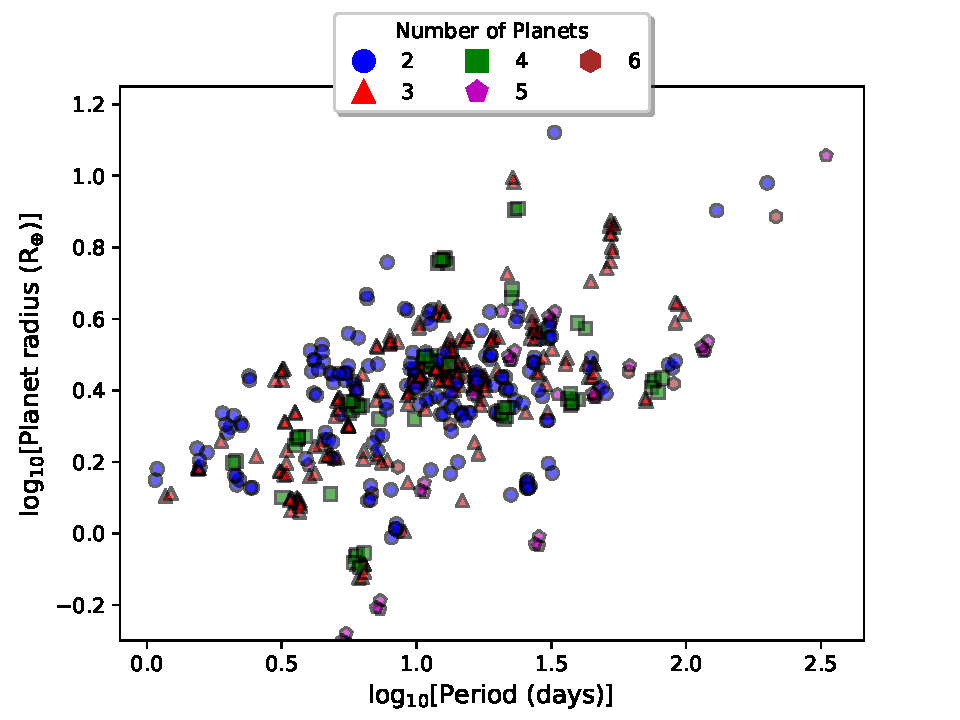
\includegraphics[width=\textwidth]{img/R_P-plot_numP1.pdf}
 	  	 \caption{Radius distribution as a function of period for the simulated TESS objects where the colour and shape corresponds to the multiplicity of the system.}
 	  	 \label{fig:RP_plot_temp_multi}
\end{figure}
	\newpage Figure \ref{fig:skymap_TESS} shows a sky map in the ecliptic frame of the simulated TESS objects and the number of times they are observed. The green area shows the approximate range where CHEOPS are able to observe the objects.  As expected, the systems in the ecliptic poles are observed the most times and most objects in the CHEOPS range are only observed once.

\begin{figure}[h!]
	\centering
	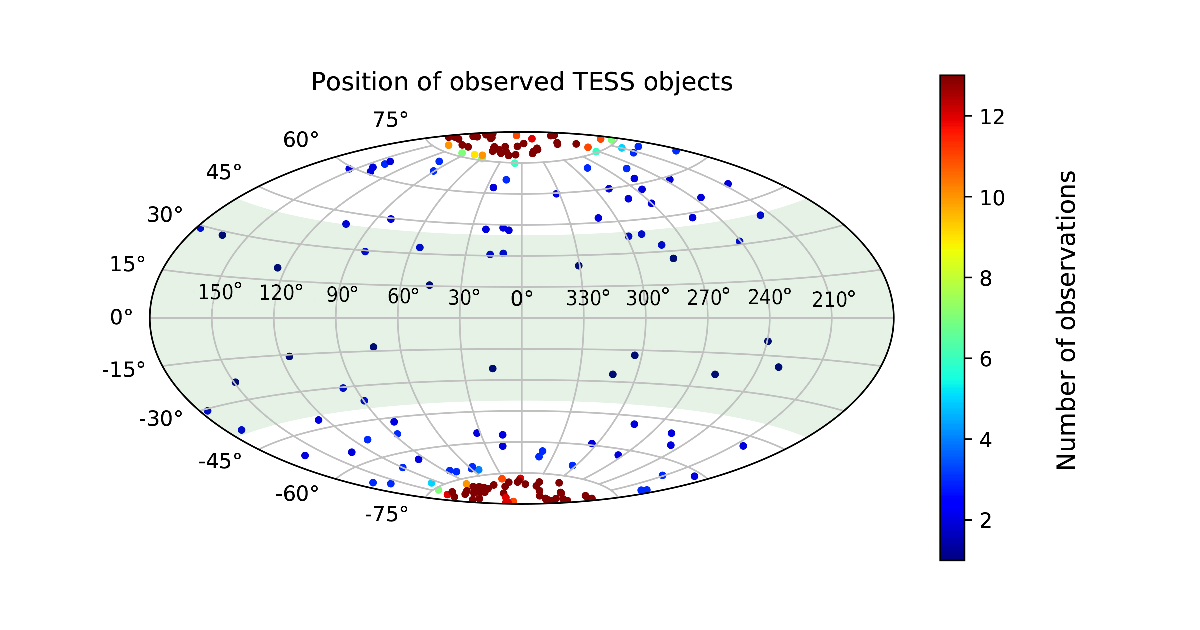
\includegraphics[width=\textwidth]{img/skymap_TESS_numObs_new.pdf}
	  \caption{Position of each observed objects in the ecliptic frame, colour-coded to show the number of times the object is observed by TESS. The green region corresponds to the part of the sky that CHEOPS will be able to observe.}	
	  \label{fig:skymap_TESS}	
\end{figure}\newpage
\section{Simulations of Ofir systems}
	Figure \ref{fig:ampl_ofir} shows the distribution of TTV amplitudes of the objects from the Ofir catalogue. In this histogram, all systems with amplitude lower than the error are filtered out as they would be undetectable and thus not of interest in this paper. It is clear that many systems show a small TTV signal but there are a significant portion of systems which show a higher amplitude. The error bars for each bin are approximated to be $\epsilon = \sqrt{N}$ where $N$ is the number of planets in the bin.
\iffalse
\begin{figure}
  \centering
  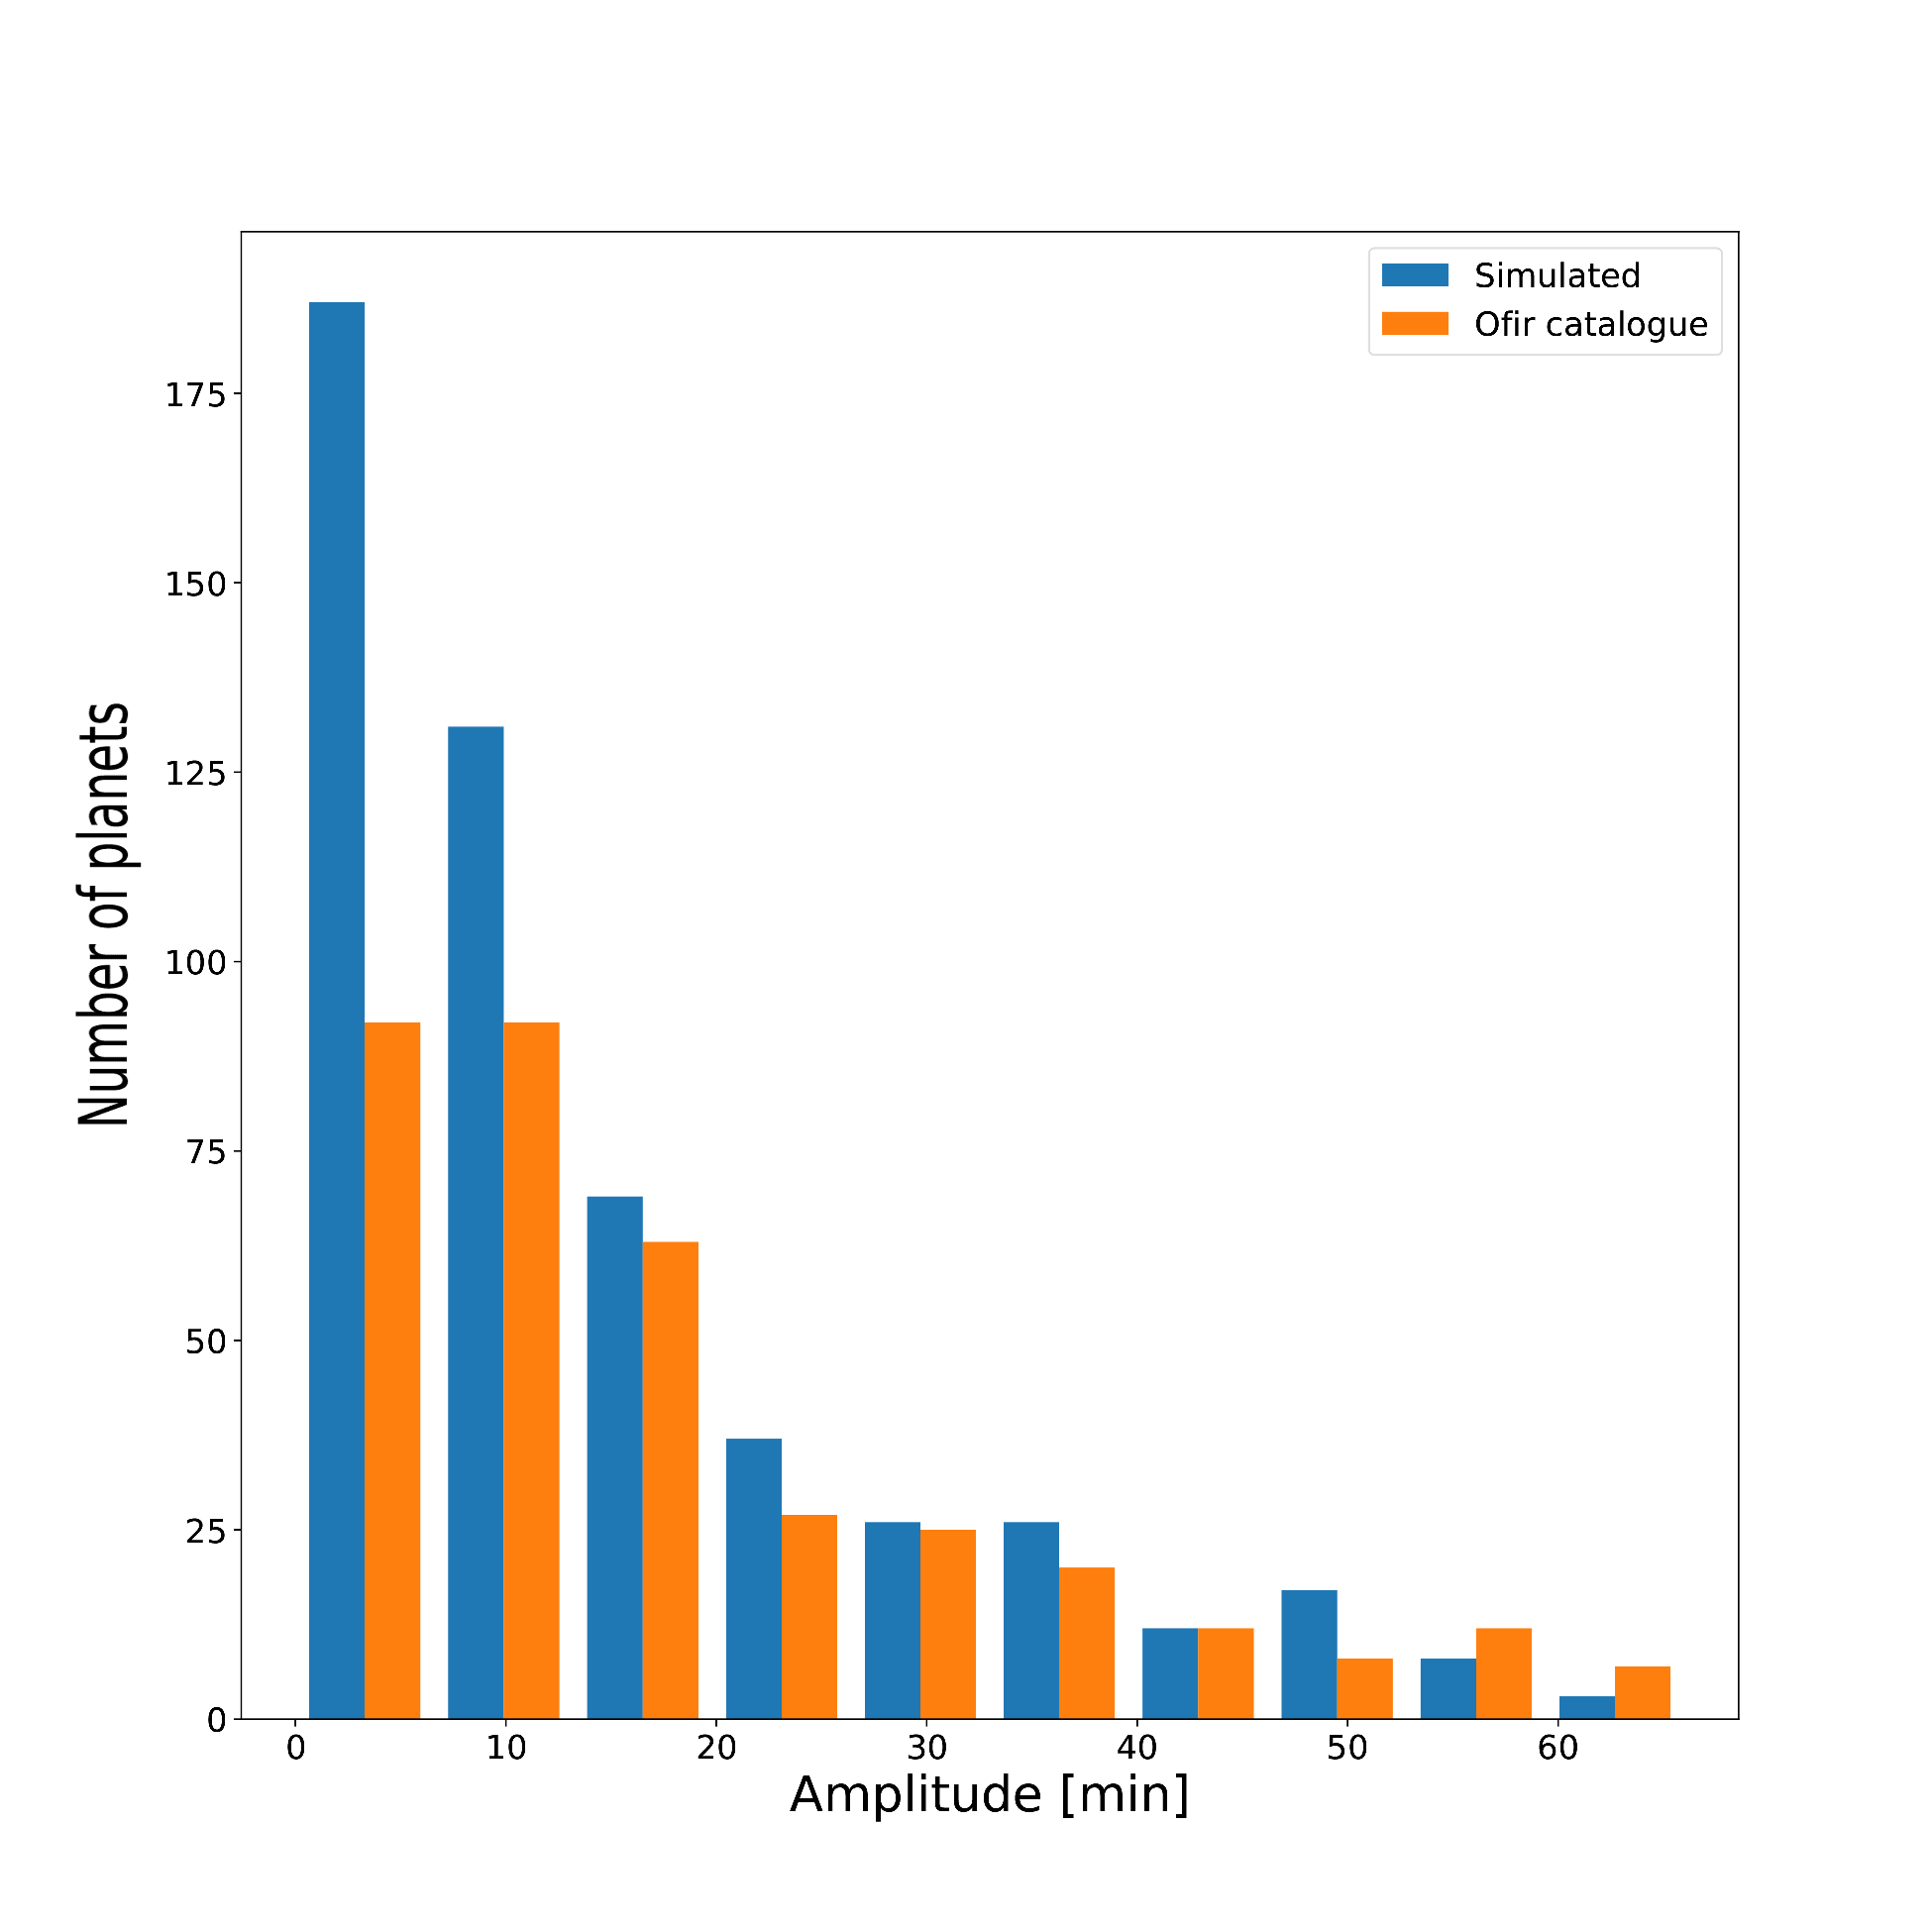
\includegraphics[width=0.5\linewidth]{img/histo_amp_both2.pdf}		
  \caption{Histogram of amplitudes obtained from simulating Kepler systems selected by Ofir et al. and the corresponding amplitudes from Ofir et al.}
   \label{fig:ampl_ofir}
\end{figure}
\fi
\begin{figure}
\centering
\begin{minipage}{.5\textwidth}
  \centering
  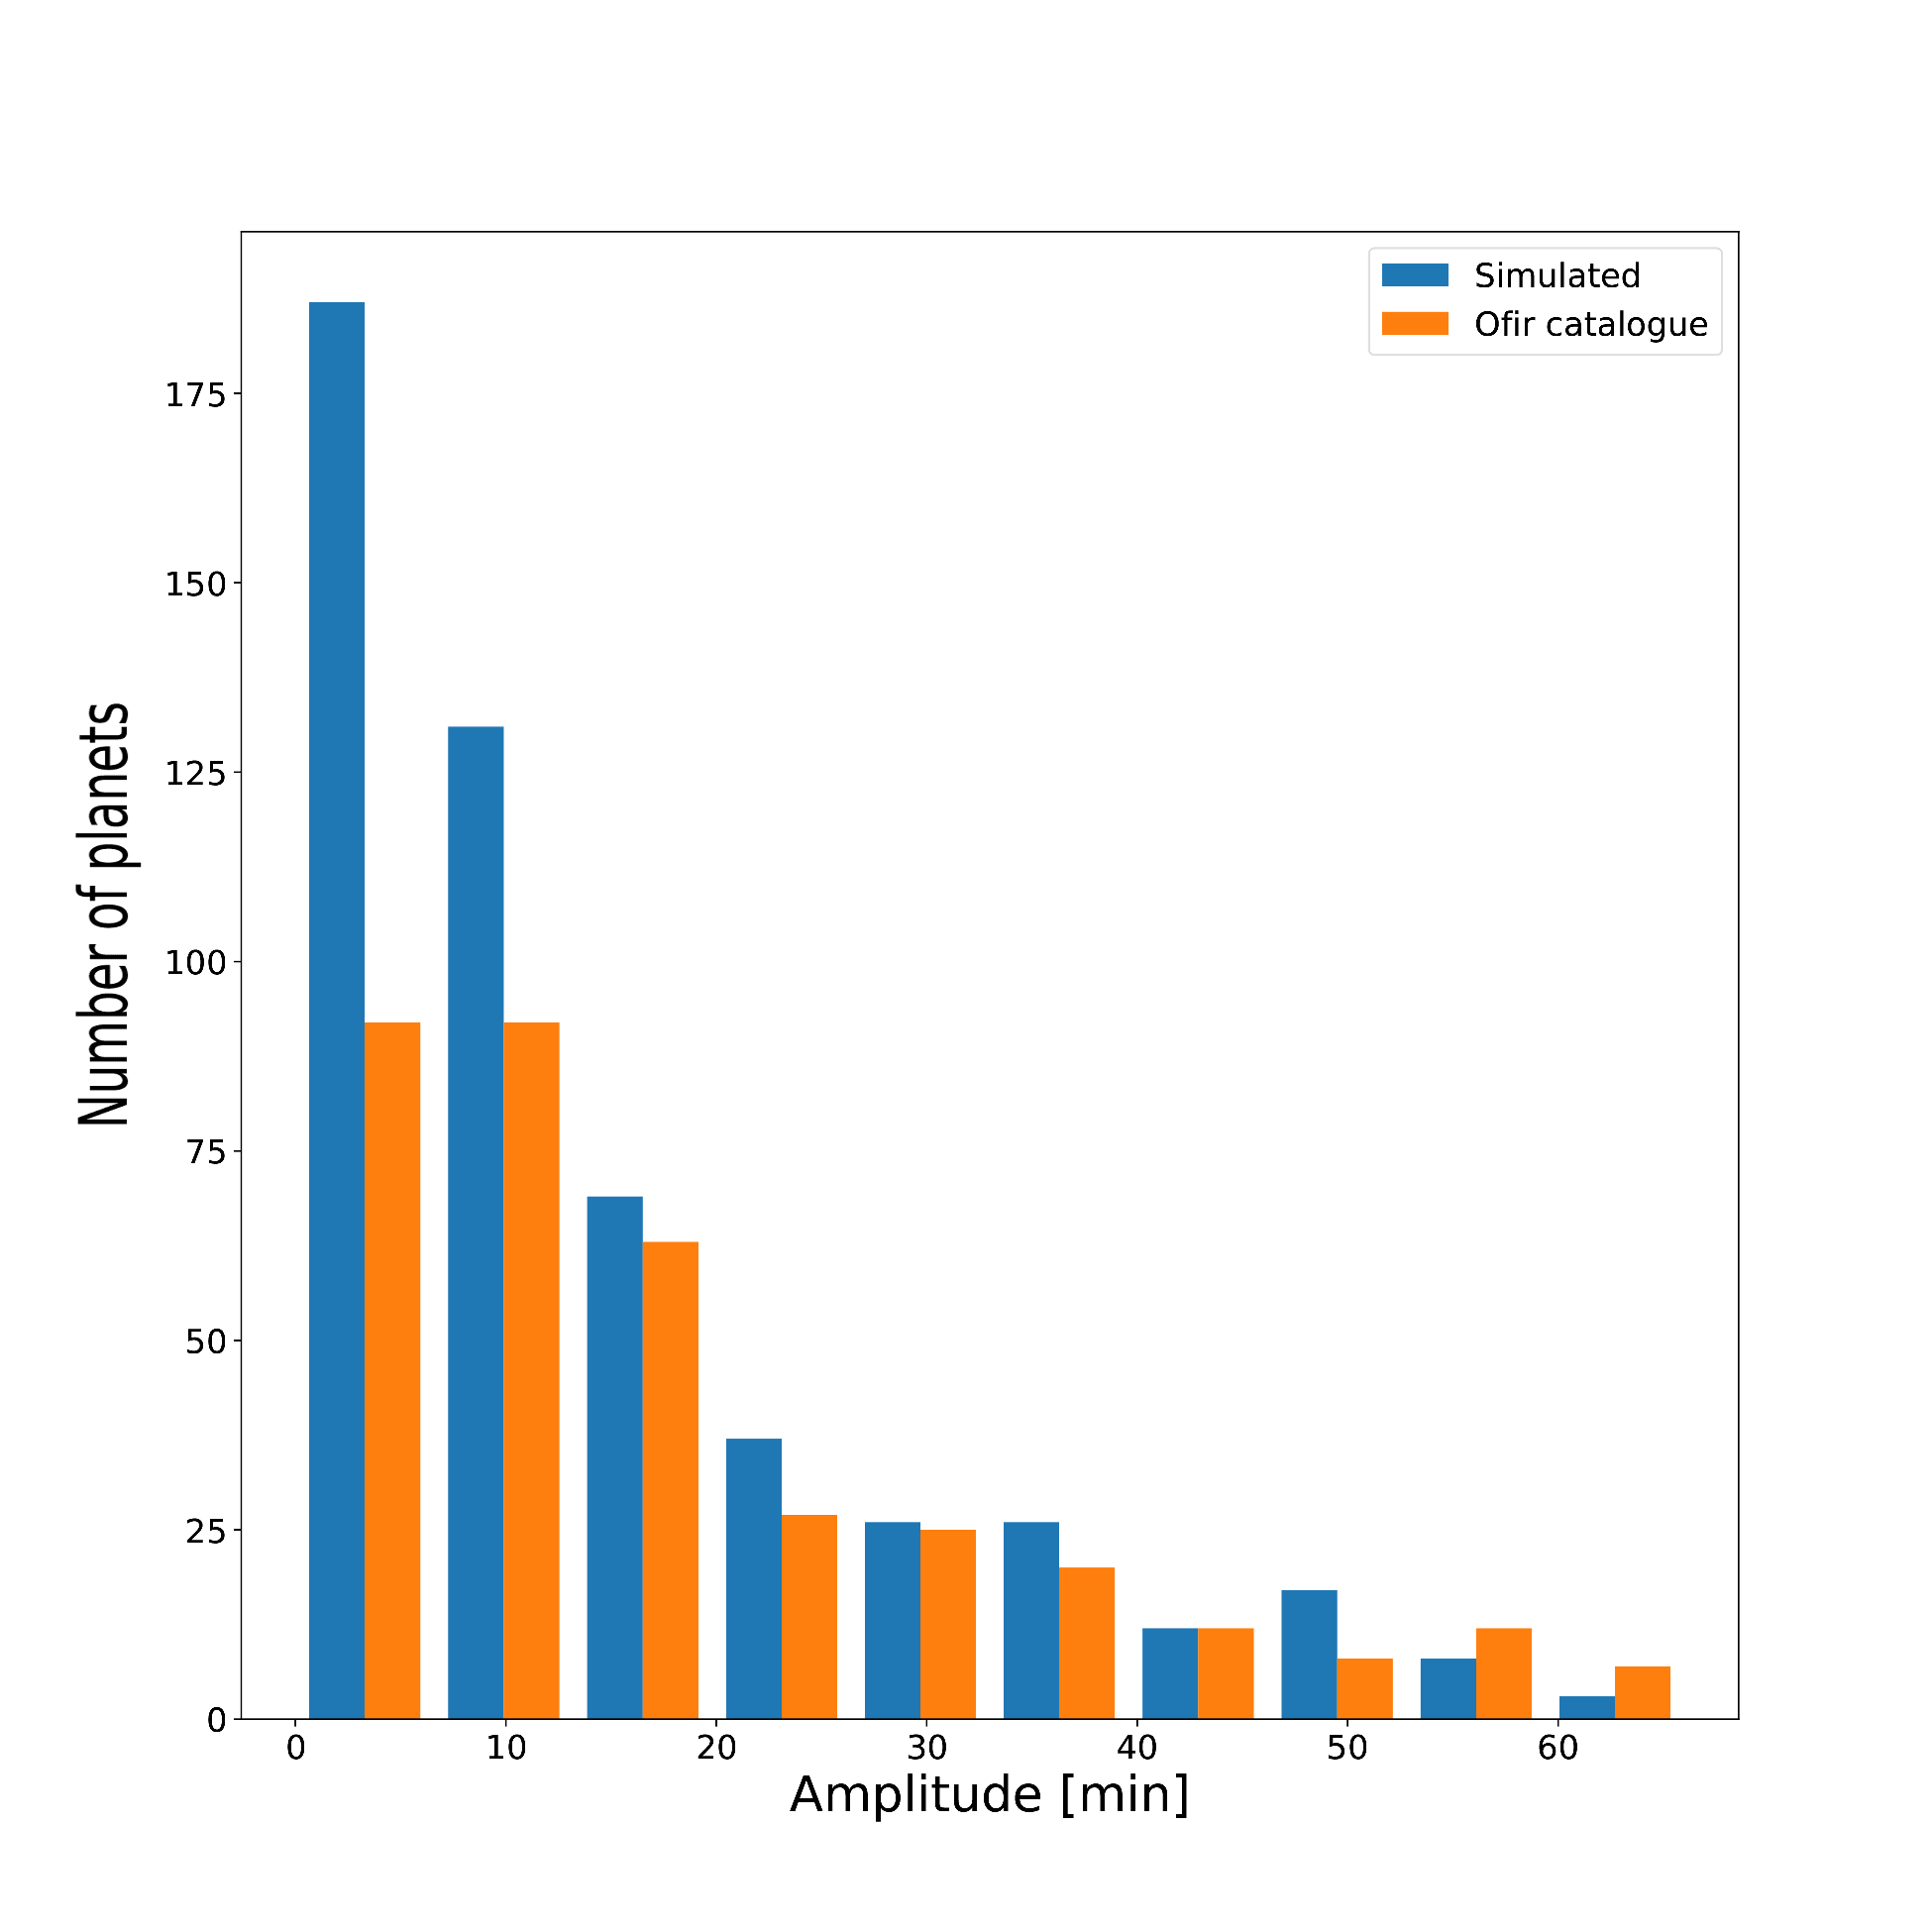
\includegraphics[width=0.9\linewidth]{img/histo_amp_both2.pdf}
  
 

\end{minipage}%
\begin{minipage}{.5\textwidth}
  \centering
  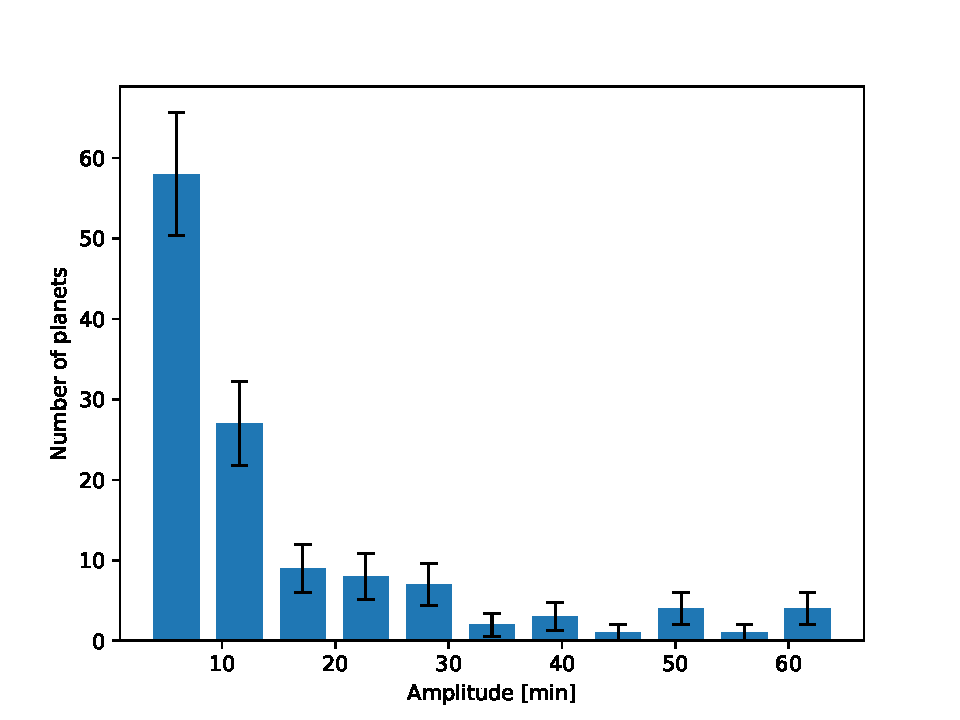
\includegraphics[width=1\linewidth]{img/ampl.pdf}
  

\end{minipage}
\caption{Left panel: Histogram of the amplitudes of the simulated Kepler systems selected by Ofir et al. and the amplitudes of these systems from the results of Ofir et al. Right panel: Histogram of the amplitudes of the simulated TESS objects}
\label{fig:ampl_ofir}
\end{figure}

\section{TTV signals from TESS objects}
	Figure \ref{fig:TTV1} shows an example of a system observed over a short duration where there is a curvature but due to the short timescale the TTV amplitude is smaller than the error. This system may show a TTV signal if observed for a longer time. The same figure shows a TTV signal for a system at one of the ecliptic poles where the variation is clearly visible. The zero level corresponds to the average transit time in order to see the variations more clearly. The distribution of TTV amplitudes are found in figure \ref{fig:ampl_ofir} where amplitudes below the error are filtered out as they would not be detectable and thus not of interest in the paper. It is easy to see that low or no TTV signals dominate but there are some planets showing substantial TTV signals. The location in the sky of these objects are shown in figure \ref{fig:skymap_amp}. Many planets at the ecliptic poles show some form of TTV signal but few planets outside do. This is due to the short observation period outside the poles. In the range that CHEOPS are able to observe about 4 out of 52 systems contains at least one planet showing a TESS detectable TTV signal. At the ecliptic poles 30 of 105 planets show a TESS detectable TTV signal. Over the whole sky 121 out of 474 planets in 189 systems show a TESS detectable TTV signal. 
	
\begin{figure}
\centering
\begin{minipage}{.5\textwidth}
  \centering
  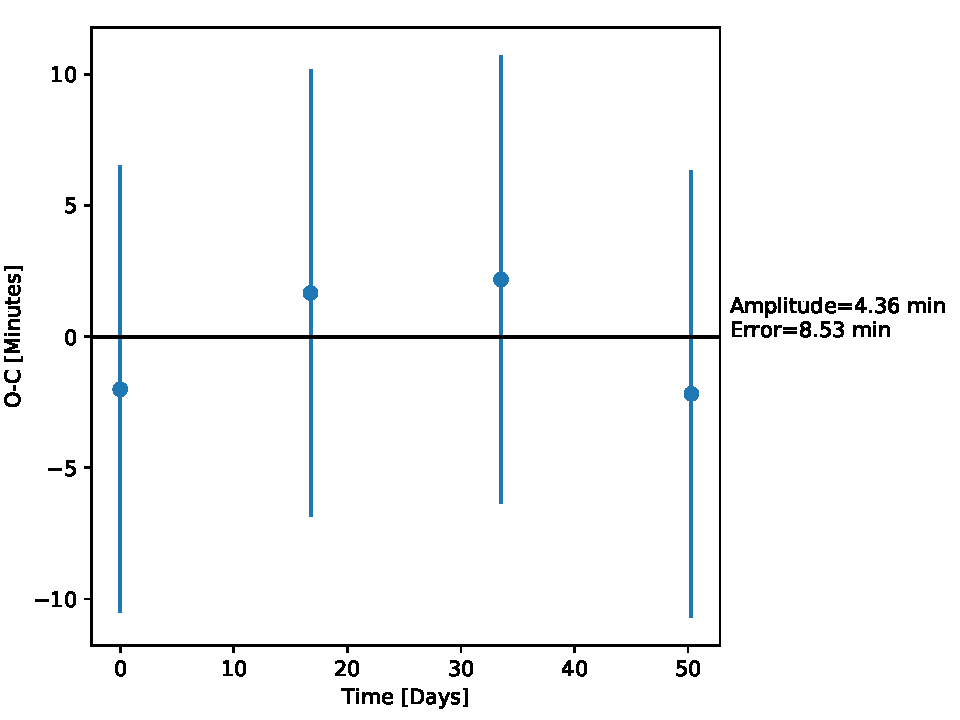
\includegraphics[width=1\linewidth]{img/20_2.pdf}
 

\end{minipage}%
\begin{minipage}{.5\textwidth}
  \centering
  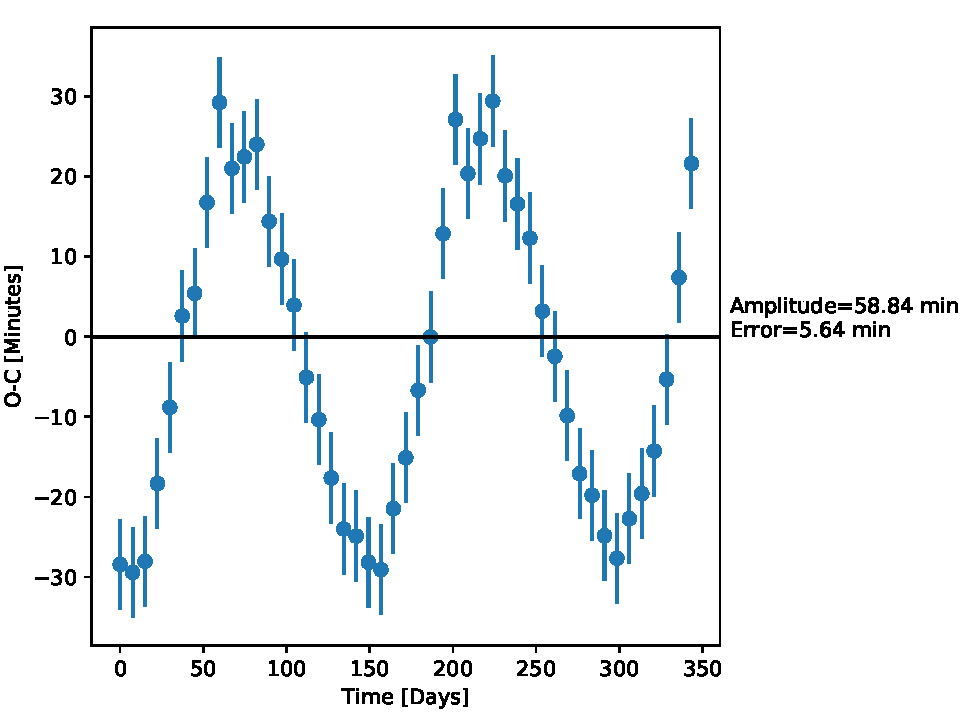
\includegraphics[width=1\linewidth]{img/247_1.pdf}
  

\end{minipage}
\caption{Observed-Calculated transit time as a function of time. The zero level corresponds to average transit time. The left panel shows a system which is observed for a short time which may show a TTV signal if observed over a longer time. The right panel shows a system located at the poles where the TTV signal are clearly seen.}
\label{fig:TTV1}
\end{figure}

\begin{figure}[h!]
 	 \centering
	  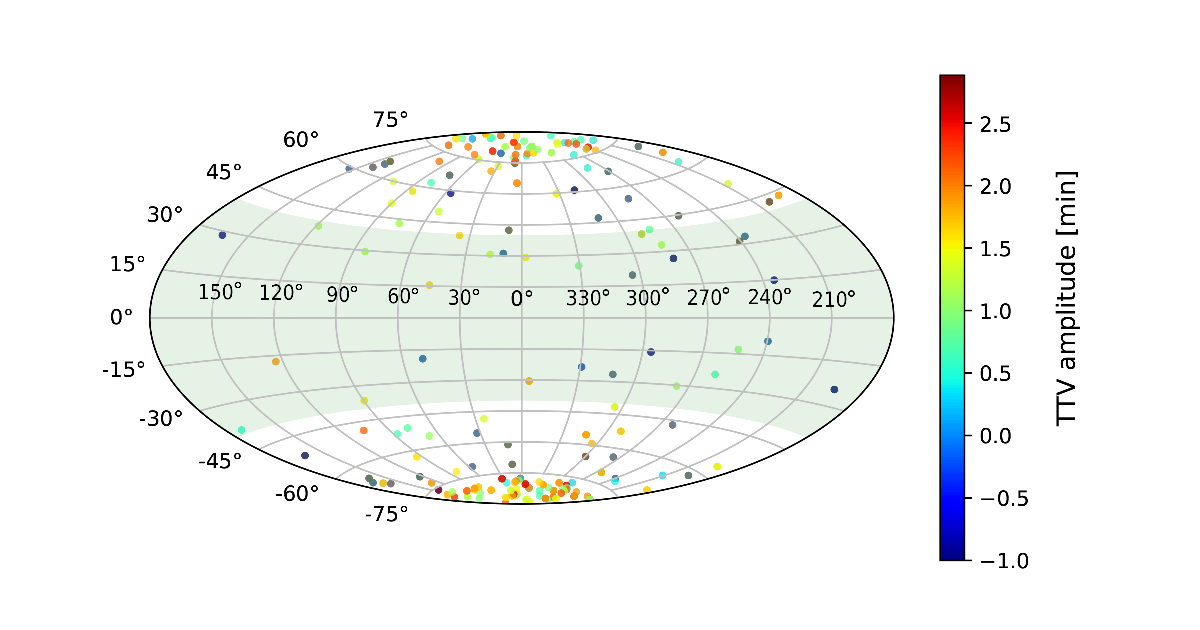
\includegraphics[width=\textwidth]{img/skymap_TESS_amp_-1_new.pdf}
	  \caption{Position in the sky in the ecliptic frame and the TTV amplitude.}
	 \label{fig:skymap_amp}
\end{figure}
\section{Error analysis}
		Figure \ref{fig:amp_error} shows the amplitude of the systems as a function of the error of the amplitude. Also shown is a line where y=x where the amplitude is equal to the error. The systems with an amplitude lower than the error cannot be considered as the signal can be due to noise.
\begin{figure}
 	 \centering
	  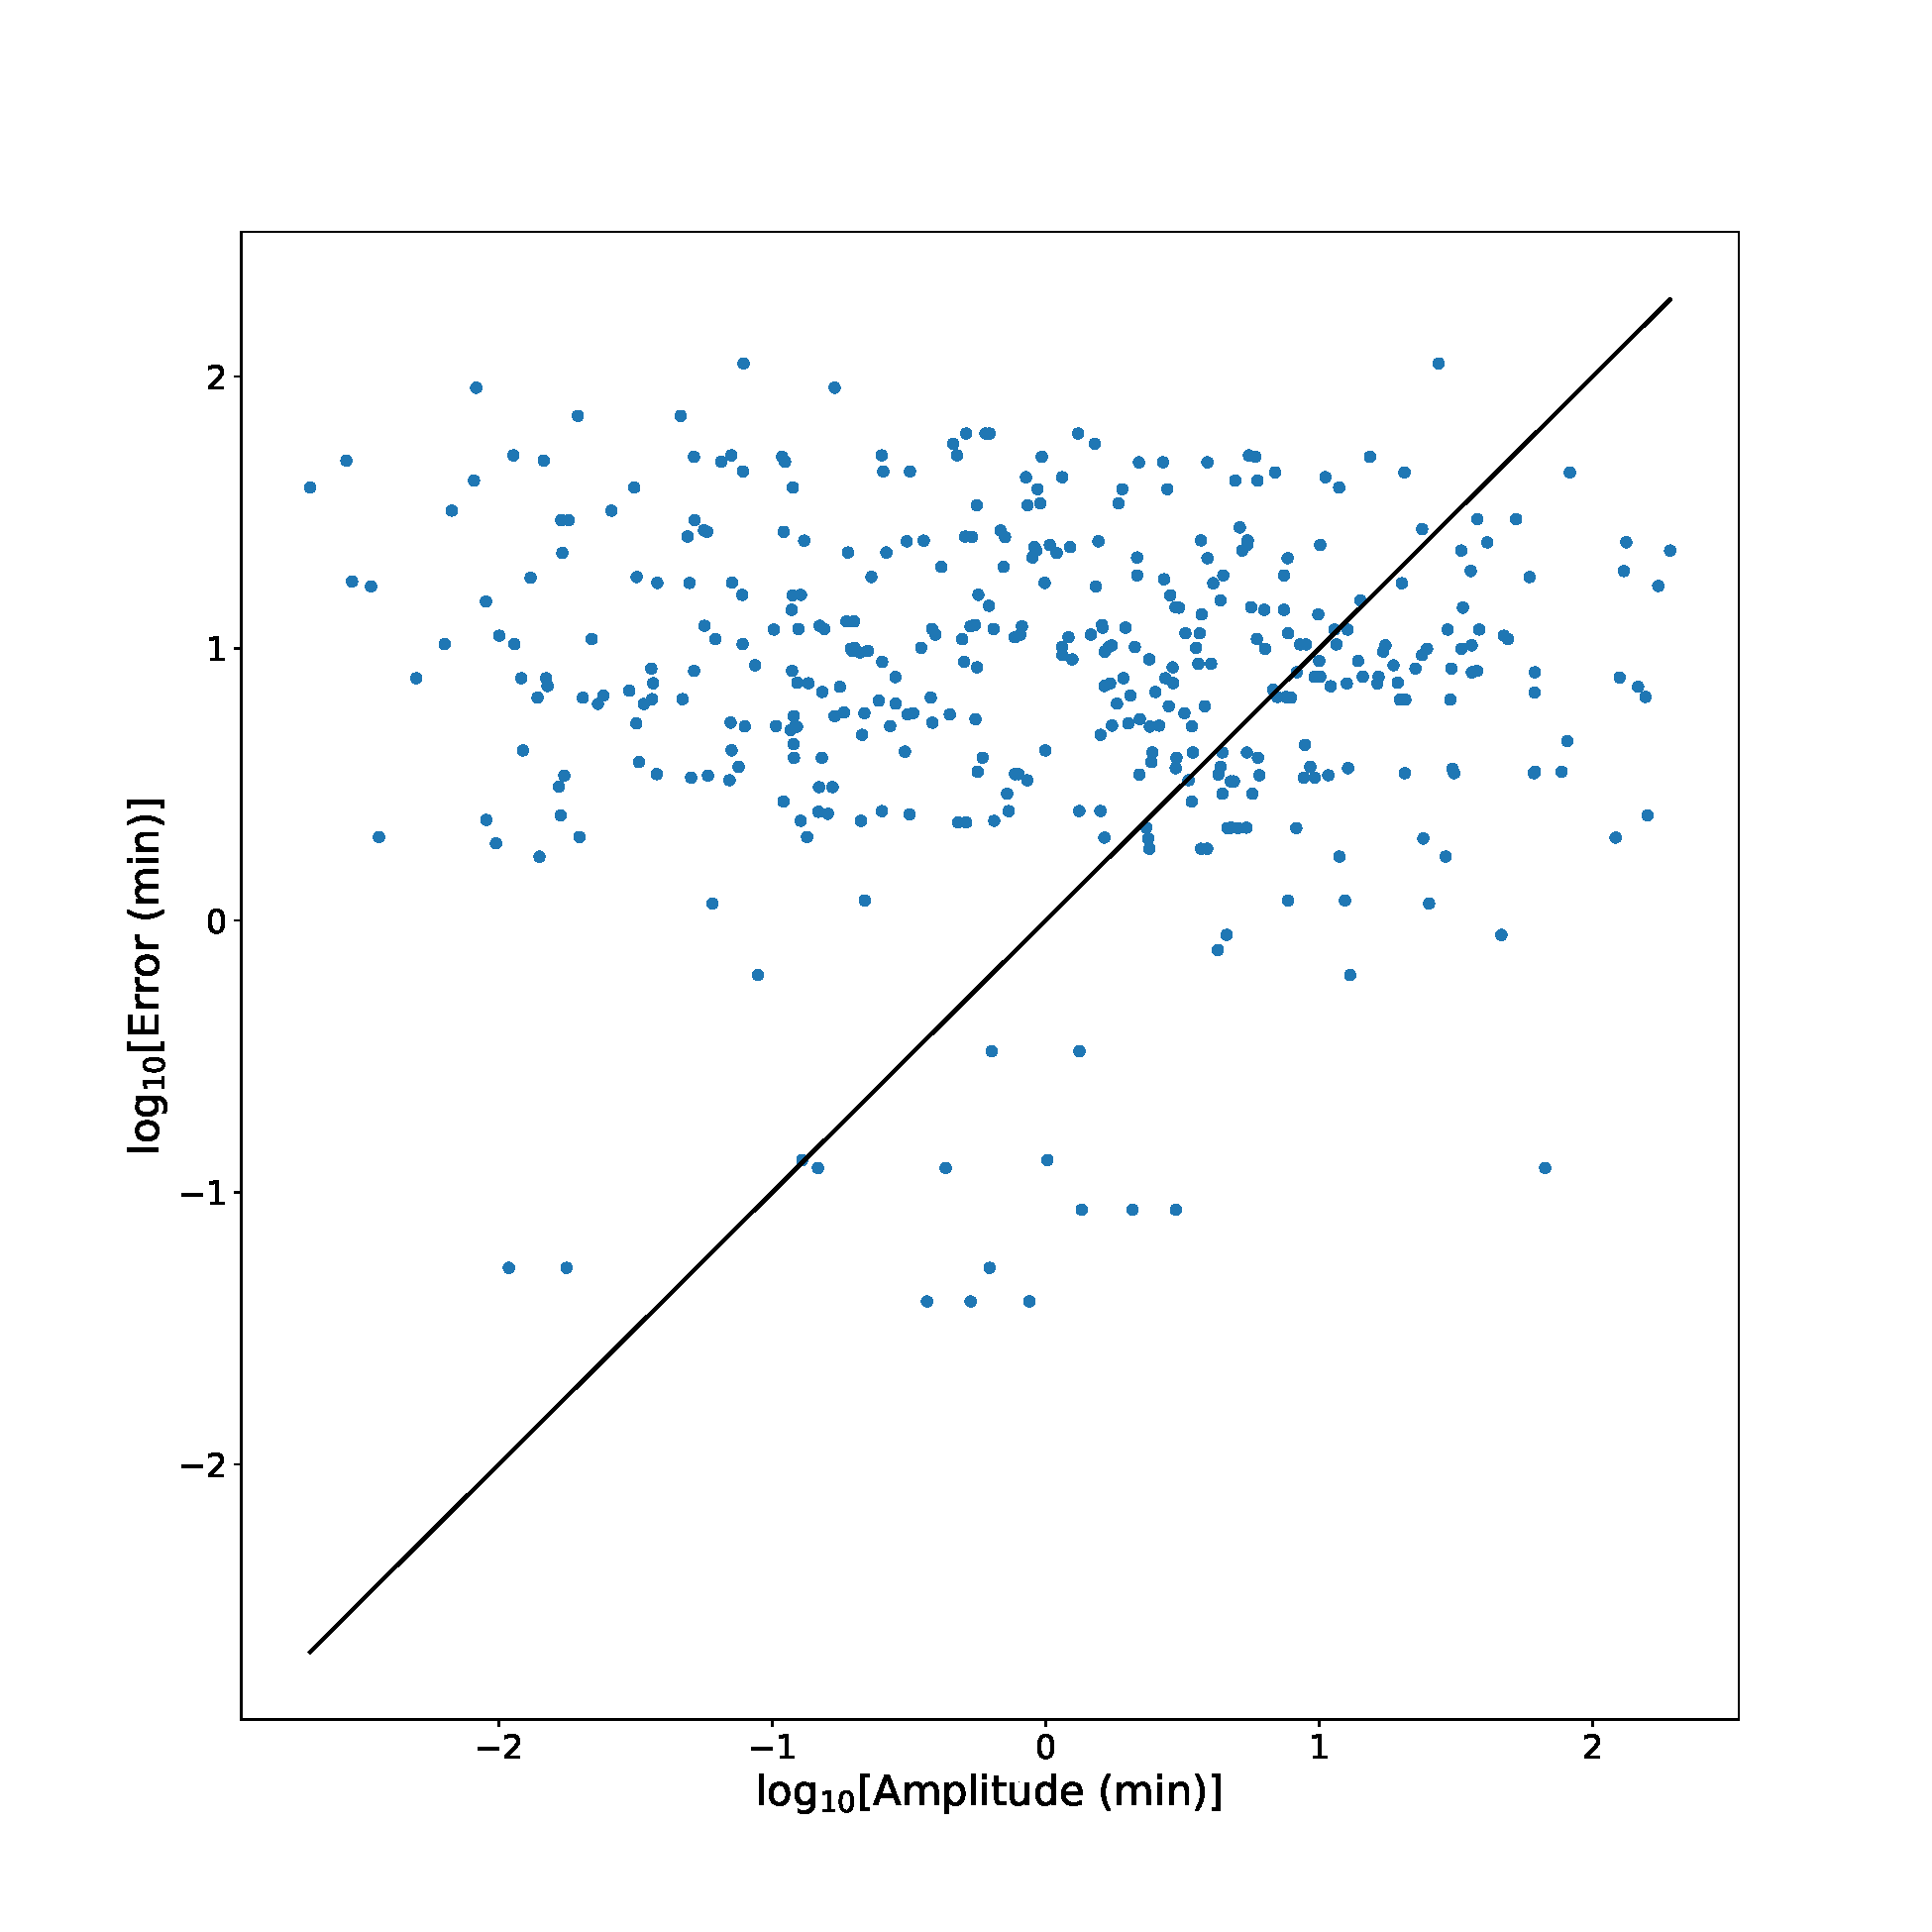
\includegraphics[width=\textwidth]{img/ampErrorLog.pdf}
	  \caption{Amplitude of the TTV signal plotted against the error where y=x is marked with a black line.}
	 \label{fig:amp_error}
\end{figure}
\section{Stability simulations}
	Figure \ref{fig:stability_sim} shows two examples of the results from the stability simulations. For all stability tested systems most  have not shown any instability within $10^5 / 10^6$ years. The systems were chosen from the separation obtained from the Hill radius where a lower separation means a higher chance of instability. Each system is simulated for 10 million orbits of the planet with the highest period. This creates a situation where most systems are simulated for $10^5$ to $10^6$ years. A few systems did eject a planet which  probably is the result of an close encounter. These systems were then re-simulated using IAS15 which showed that they were in fact stable and the ejection was a result from WHFast not being able to handle the close encounters. It can be noted that all of the planets are very close to the host star. This is a result from how the semi-major axis is calculated, as most planets in this paper have a short period the semi-major axis is small which results in very closely packed systems.

\begin{figure}
\centering
\begin{minipage}{.5\textwidth}
  \centering
  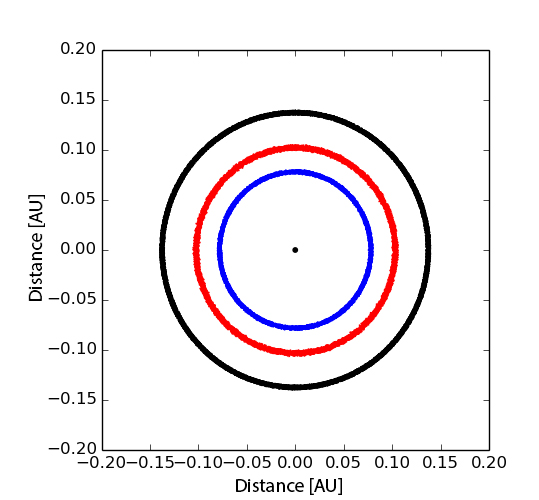
\includegraphics[width=1\linewidth]{img/180.jpg}
 

\end{minipage}%
\begin{minipage}{.5\textwidth}
  \centering
  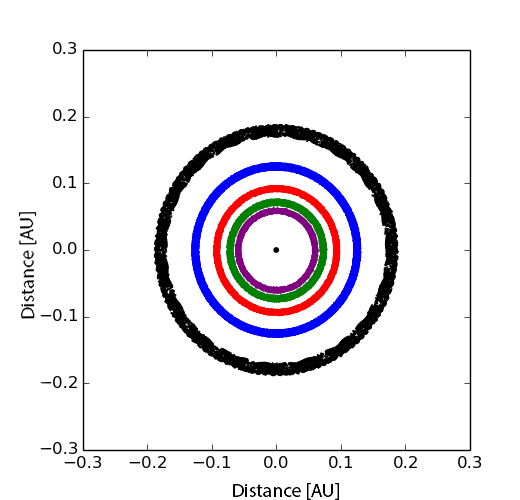
\includegraphics[width=1\linewidth]{img/320.jpg}
  

\end{minipage}
\caption{Stability simulations for two systems over $10^6$ years. Left panel: Orbits of the planets in a three planet system. Right panel: Orbits of the planets in a five planet system}
\label{fig:stability_sim}
\end{figure}

\section{Amplitude dependence on time}
	A system was selected where the TTV signal was as close to a sine curve as possible. This curve can be seen in the left panel of figure \ref{fig:ampTime}. The resulting amplitude curve with the corresponding analytical amplitude can be seen in the right panel in figure \ref{fig:ampTime}. The TTV curve is close to a sine curve but it is slightly shifted to the right, despite this, both curves show the same behavior. Initially the curve decreases with very low curvature. After the peak the curve increases again and after it goes past the initial point the amplitude increases greatly until it plateaus. As the TTV curve is not a perfect sinusoidal curve the analytical amplitude is correct for low time but increases too quickly and overshoots the simulated value. 
	
	As the TTV amplitude increases over time a system not showing TTVs on a short timescale might show TTVs on a longer timescale such as when observed by CHEOPS. This gives an estimation of which systems are interesting and can be selected for follow up observations.

\begin{figure}
\centering
\begin{minipage}{.5\textwidth}
  \centering
  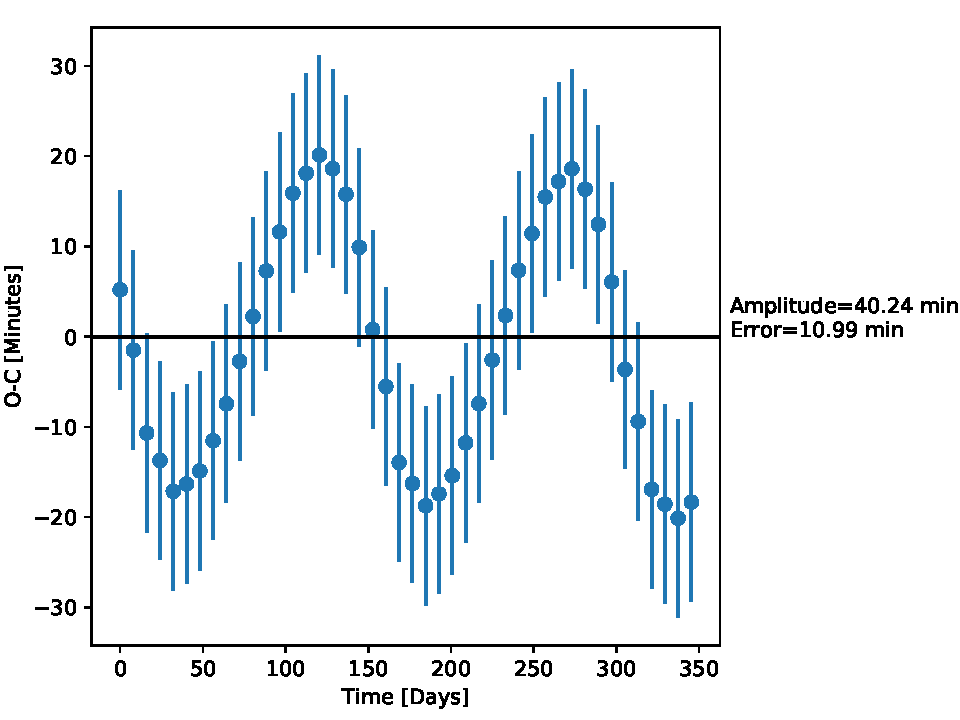
\includegraphics[width=1\linewidth]{img/62_1_new2.pdf}
 

\end{minipage}%
\begin{minipage}{.5\textwidth}
  \centering
  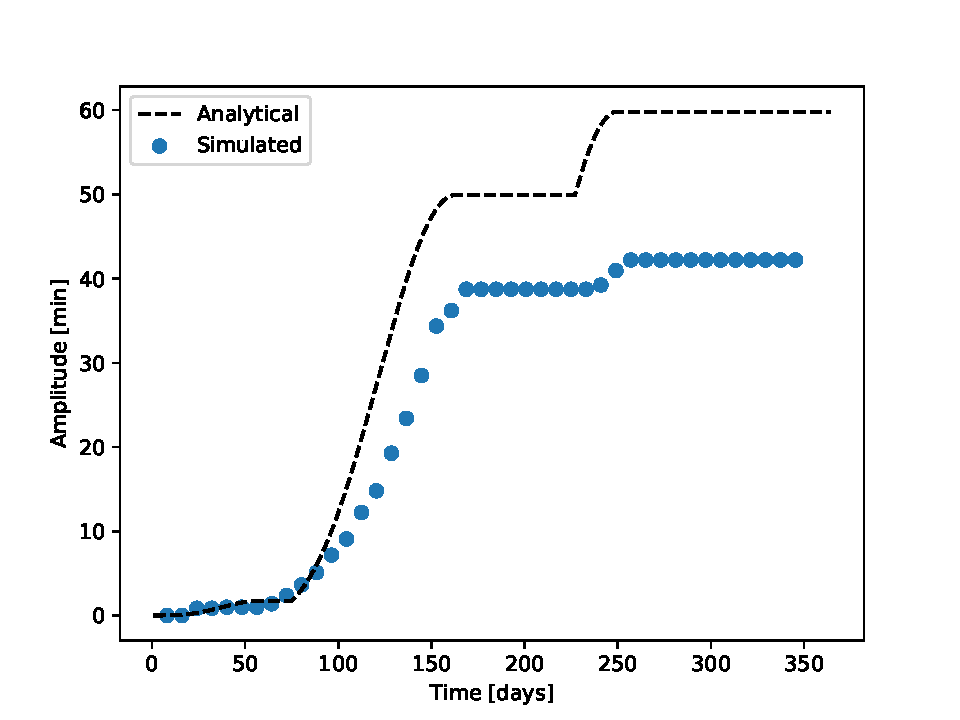
\includegraphics[width=1\linewidth]{img/62_1_new2_amp.pdf}
  

\end{minipage}
\caption{Left panel: TTV curve of selected system for amplitude analysis. Right panel: Amplitude curve of selected system where the simulated amplitude are represented by blue dots and the analytical amplitude by the dotted line.}
\label{fig:ampTime}
\end{figure}



\section{Objects in CHEOPS observation range}
	In the left panel in figure \ref{fig:CHEOPS_perRatio} the TTV amplitude of one planet in a system is correlated to the radius of the adjacent planet in the system. This is to see a relation between TTV amplitude of one planet and radius/mass of another as the TTV amplitude is dependent on the mass of the other planet. It is shown that the amplitude increases for systems where the period ratio is close to 1 and decreases for higher ratios. Also in general the amplitude is lower for lower radius with the highest at about $2.5\; \mathrm{R_{\oplus}}$ which might be due to that there are a large amount of planets in this radius range which increases the chances of seeing a high TTV amplitude. In the right panel the TTV amplitude increases for low period ratio and decreases for higher. At around period ratio = 2 there are a visible peak in amplitude which originates from the 2:1 resonance. In total 3000 systems were created which contains 6800 planets. Of these, 6798 planets showed some form of TTV signal and out of these 3291 planets showed a CHEOPS detectable TTV signal.
	
	In figure \ref{fig:CHEOPS_prob} the probability to find a detectable TTV signal during 1 year of observations based on the planet radius and period ratio is shown. As expected low period ratio gives a higher probability and higher period ratio show very low probability to get a detectable signal. From these results, if a planet with, for example, radius around $2.5$ R$_{\oplus}$ and a period ratio of 3 is found there are a large probability that that planet will show a detectable TTV signal.
\begin{figure}
\centering
\begin{minipage}{.5\textwidth}
  \centering
  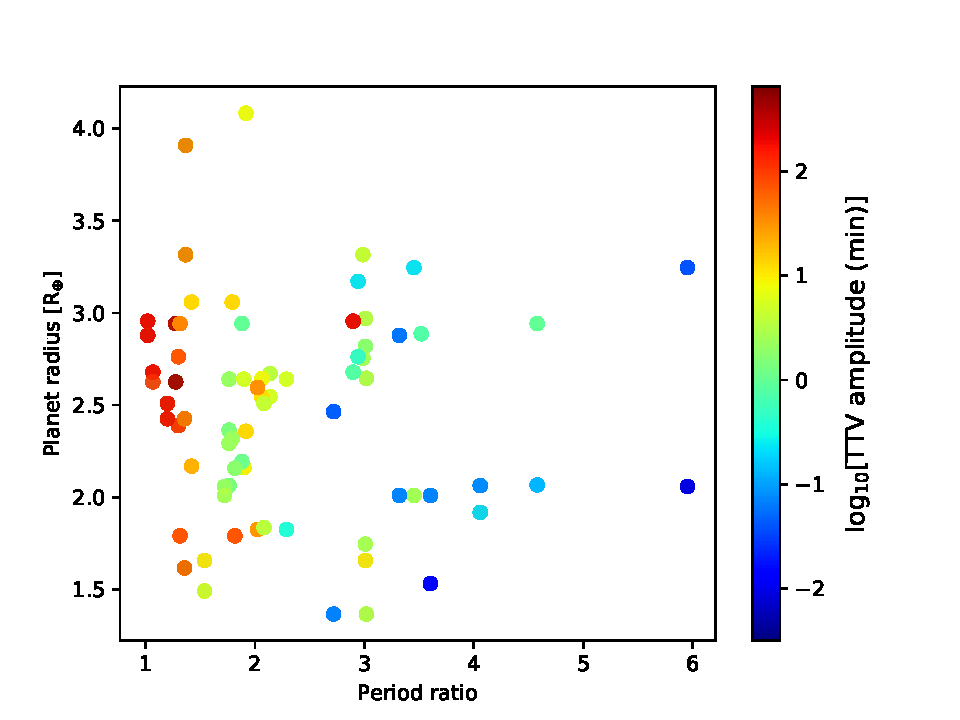
\includegraphics[width=1\linewidth]{img/perFracRad.pdf}
 

\end{minipage}%
\begin{minipage}{.5\textwidth}
  \centering
  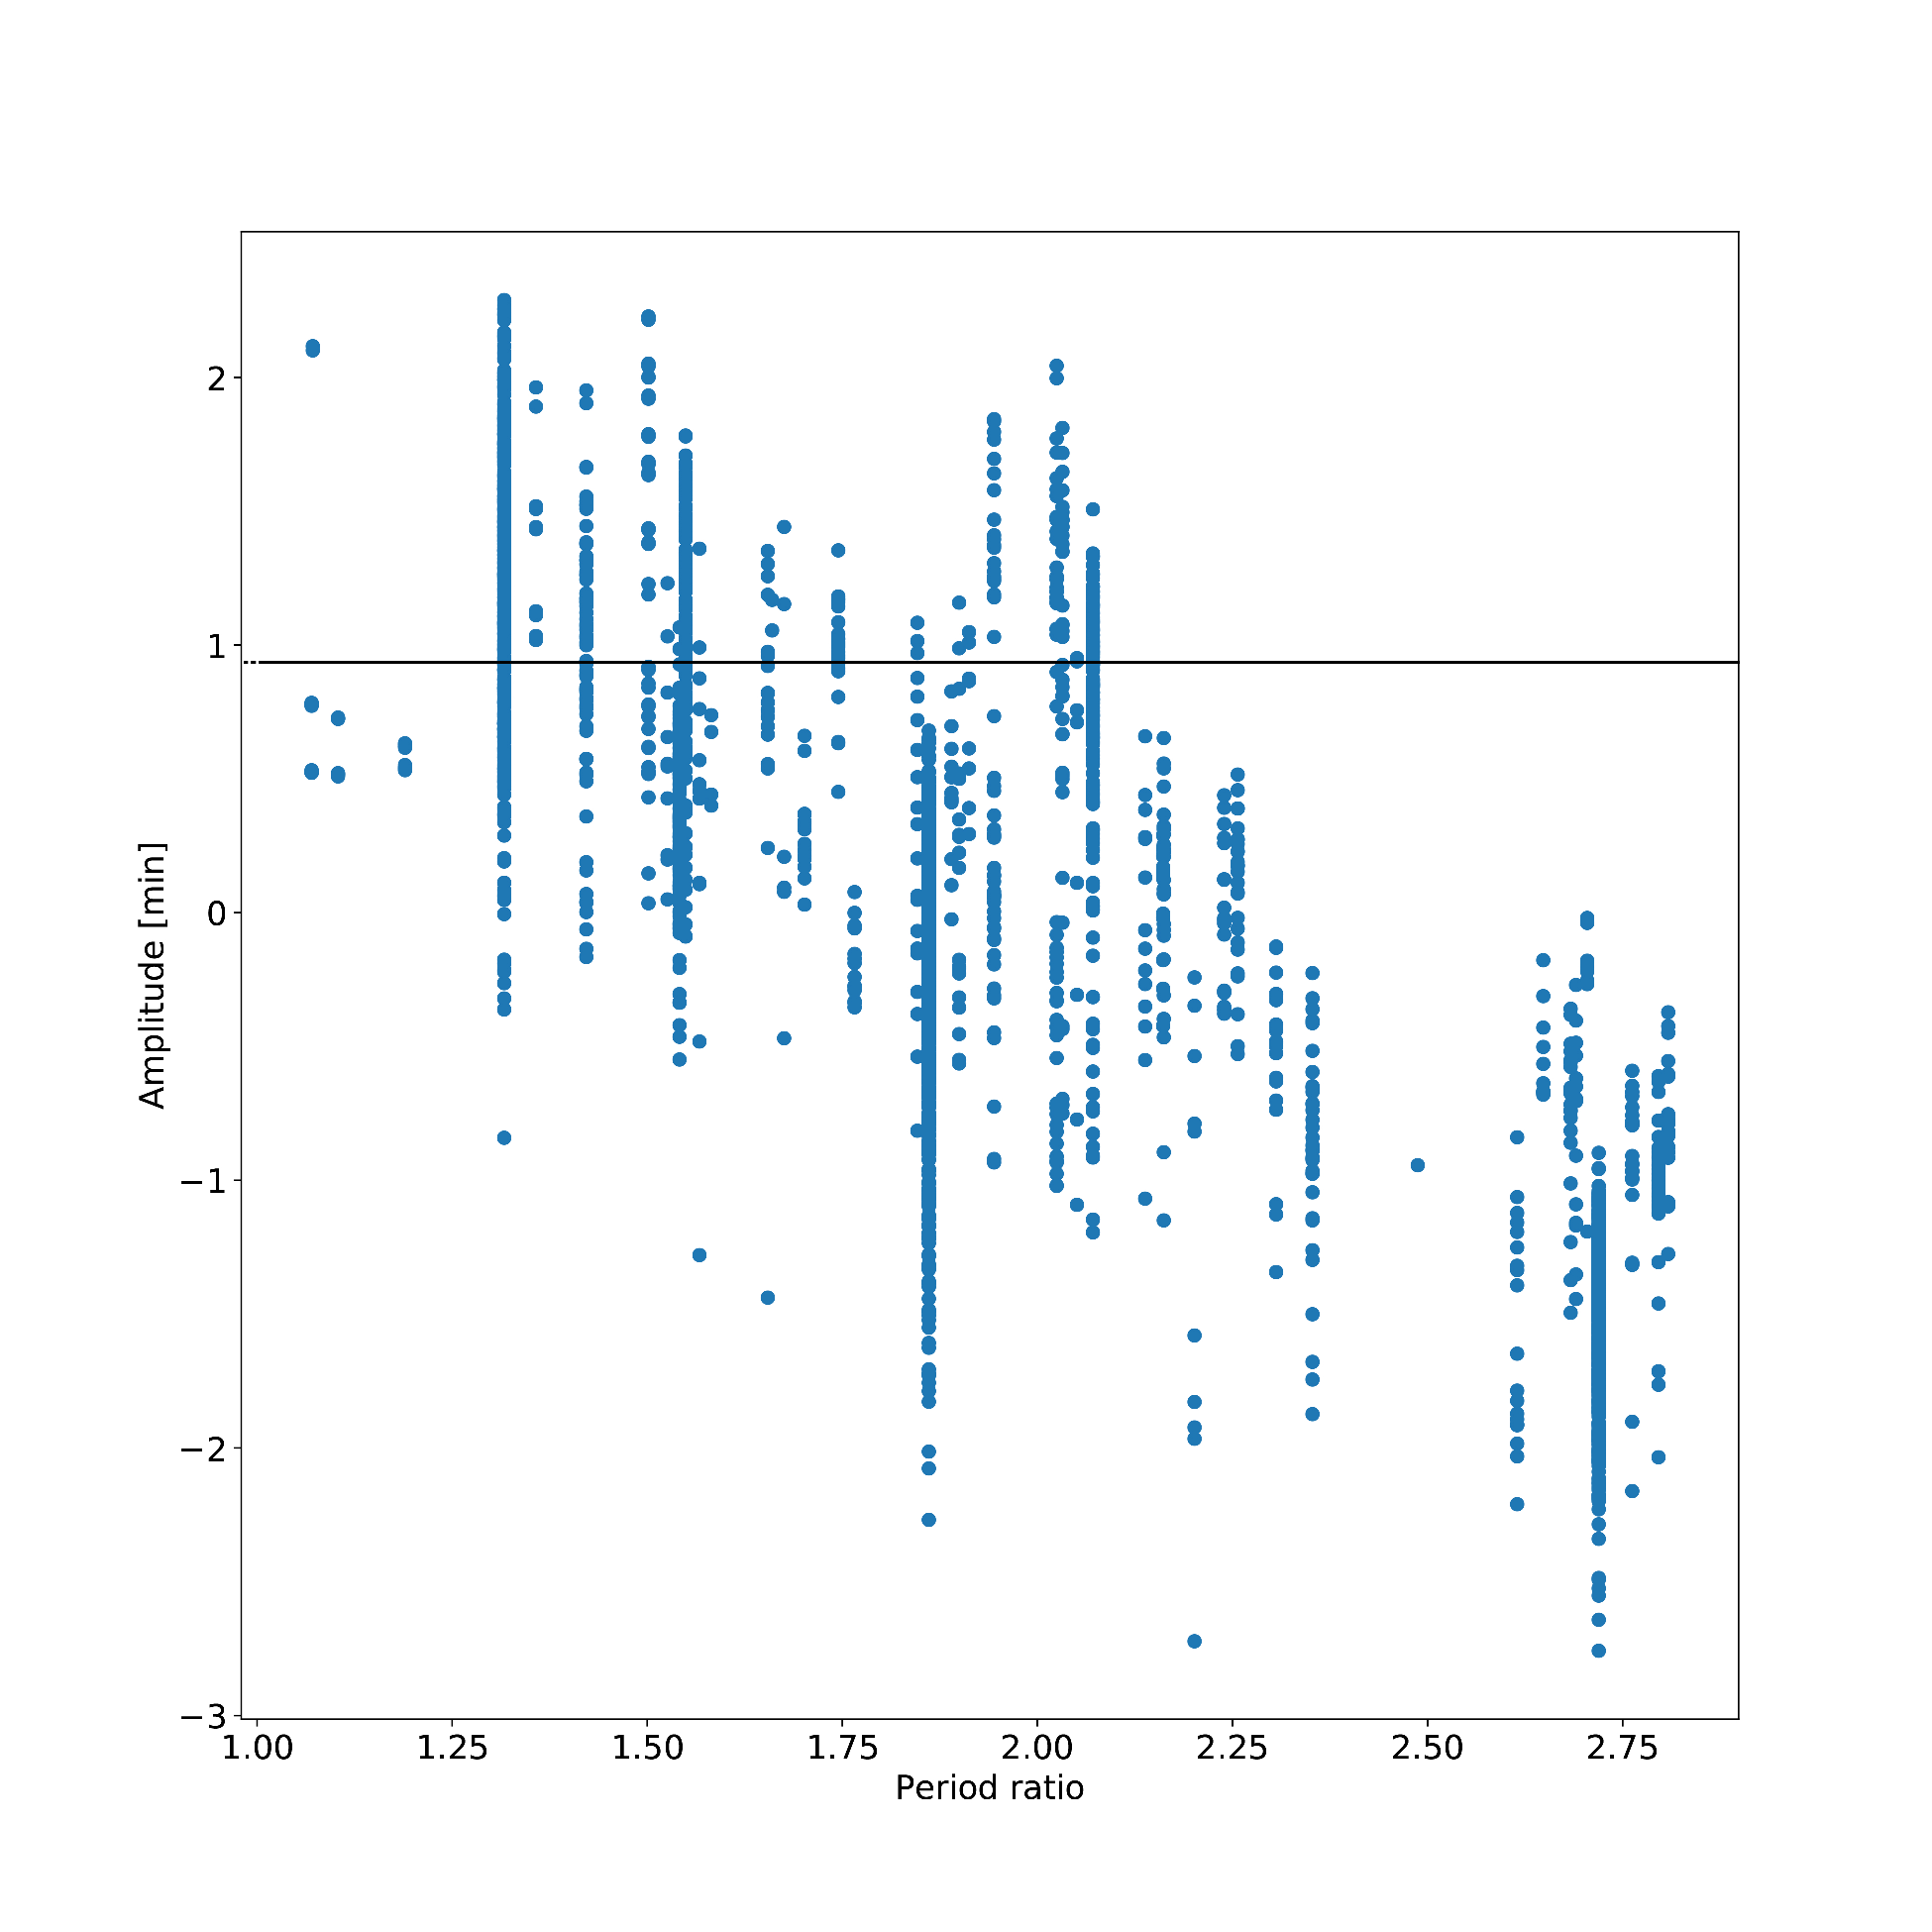
\includegraphics[width=1\linewidth]{img/ampPratDouble_3_line.pdf}
  

\end{minipage}
\caption{Left panel: Planet radius plotted against period ratio where the amplitude of the TTV signal is color coded. Right panel: Amplitude plotted against period ratio where the median TTV error is represented as a black horizontal line.}
\label{fig:CHEOPS_perRatio}
\end{figure}

\begin{figure}
\centering
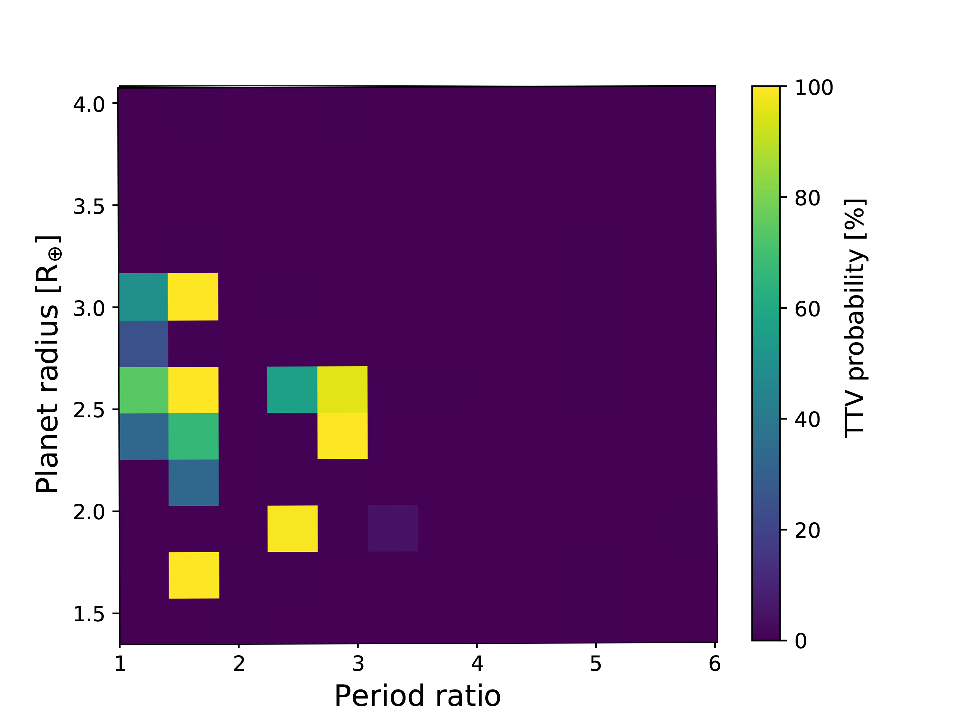
\includegraphics[width=0.7\textwidth]{img/2dhist3_new.pdf}
\caption{2d histogram of detectable TTV probability depending on planet radius and period ratio.}
\label{fig:CHEOPS_prob}
\end{figure}

\iffalse
\begin{table}[!h]
\caption{Example table from template}\smallskip
\label{table:1}
\centering  
\begin{tabular}{lrrc}
\hline\hline  
\smallskip
Id of star & I &  V & Var.? \\
\hline
1234 & 15.6 & 17.3 & No \\
5677 & 13.4 & 12.3 & Yes\\
\hline
\end{tabular}
\end{table}
\fi

\chapter{Discussion}
	These results may be used to give an approximated upper limit of how many systems in a given sample will show TTV signals. The systems can be observed in more detail by, for example, the CHaracterising ExOPlanets Satellite, CHEOPS, or the James Webb Space Telescope, JWST. CHEOPS are not able to measure stars at the poles and are limited to the sky around the plane of Earth's orbit which are marked as a green area in figure \ref{fig:skymap_TESS} and \ref{fig:skymap_amp}. As TESS will have coverage of the poles for the whole year many of the systems showing TTV signals will be located at the poles. The JWST on the other hand will be able to look at the poles. CHEOPS will be used to further study already found systems in order to more accurately measure the radii of the exoplanets. It can be used to obtain more transits and thus give more opportunities to measure TTVs. JWST will study the spectrum of a star and compare it to the spectrum of the same star when an exoplanet is transiting. With high enough precision this will make it possible to approximate the composition of an potential atmosphere around the exoplanet. To determine the atmosphere the surface gravity of the planet needs to be known which comes from the mass and radius of the planet. The radius can be obtained from the transit method while the mass may be obtained from a TTV signal or the radial velocity method.
	
	The way of determining the amplitude of the TTVs are very simplistic. It is simply an average of the highest and lowest value. This can be improved by some kind of fit as the TTV signals are often in the shape of a sine curve but due to time constraints this paper does not include this way of determining the amplitude.
	
	Even though these results show that CHEOPS might be able to find a planet showing TTV signals in every other system the real number is probably lower. An approximation used in this paper is that the inclination is $90^{\circ}$ for all planets. This creates systems where all planets are transiting which is not the case for real systems. Also for some TTV signals the super-period, the period of the TTV signal, is longer than the observational baseline. In these cases fitting a sinusoid is meaningless as the signal won't have time to show the full period. 
	
	The systems are checked for stability and ensure that they are realistic with WHFast, IAS15 and by comparing the distribution of amplitudes from the TESS objects with the objects from the Ofir et al. paper. Using WHFast, most systems tested for stability show no sign of instability within $10^5 / 10^6$ years. The few that do are simulated using IAS15 where they are shown to be stable and the instability from WHFast can be considered an effect of WHFast's inability to handle close encounters. The artificial systems created in this paper contain some planets which show strong TTV signals, mainly positioned in the ecliptic poles as the systems positioned here are observed for a whole year which gives many more opportunities to detect TTVs. The shape of the histogram in figure \ref{fig:ampl_ofir} are the same as in the Ofir paper. This shows that the methods of simulating systems used in this paper are viable and give reasonable results.
	
	The error calculations seem to give reasonable results \citep{2015ApJ...812L..18B}. As seen in figure \ref{fig:amp_error} many systems shows a TTV amplitude higher than the error but many systems shows a TTV amplitude lower than the error, for these systems no conclusion can be made as the signal could be true but it might as well be noise. The error is solely based on photon statistics and does not take things like cadence into consideration which would otherwise increase the errors. 
	
	The error calculation done in this paper is based on the photometry of TESS. As CHEOPS will have a larger camera than TESS the error will be of a factor 2-3 lower and thus increase the chance of a detectable TTV signal.
	
	The TTV amplitudes of objects within the CHEOPS observation range are in general low due to the short observation time of these objects. By considering figure \ref{fig:ampTime} where the amplitude is shown to increase over time and figure \ref{fig:CHEOPS_prob} where high TTV probability can be seen for systems with low period ratio and relativity high radius/mass the long term TTV amplitude may be predicted. A transiting planet with a radius of about 2.5 R$_{\oplus}$ and a period ratio of 2 should, based on the simulations in this paper, have a fairly high probability to show a detectable TTV signal. On the other hand, for a period fraction greater than 3 the probability to find a detectable TTV signal is very low.


	
	
\chapter{Conclusions}
	This paper simulated TESS objects using data from the Kepler dataset and results from the paper by \cite{2015ApJ...809...77S} on a search to predict TTV signals caused by multiple planets in the systems. The results can be seen below:
	\begin{itemize}
		\item Most of the systems showing TTV signals are positioned at the ecliptic poles. This comes from the fact that TESS has continuous coverage of the poles during the year which increases the chance to see TTVs. The amplitude grows non-linearly with time and thus a system might show very low amplitude on a short timescale but very high if observed for longer.
		\item In the range where CHEOPS is able to observe only 4 out of 52 systems included a planet with a TTV amplitude greater than the TESS amplitude error when simulated on a short timescale. Upon further analysis, 3291 out of 6800 planets showed a CHEOPS detectable TTV signal when simulated for 1 year. At the ecliptic poles where the JWST continuous viewing zones are located 30 out of 105 planets showed a TESS detectable TTV signal. Over the whole sky 121 planets out of a total 474 showed a TESS detectable TTV signal.
		\item Based on TESS observations objects around the ecliptic where CHEOPS will observe will show a low TTV signal due to the low observation time. Based on further simulations these objects may show a detectable TTV signal over a longer observation period which may be predicted based on the planetary radius and period fraction of the planets in the system.
	\end{itemize}

\section*{Acknowledgements}
This research has made use of the Kepler dataset, which is operated by the California Institute of Technology, under contract with the National Aeronautics and Space Administration under the Exoplanet Exploration Program. \vspace{0.5cm}\\
This research made use of Astropy, a community-developed core Python package for Astronomy (Astropy Collaboration, 2013).\vspace{0.5cm}\\
Simulations in this paper made use of the REBOUND code which can be downloaded freely at \url{http://github.com/hannorein/rebound}.



%\bibliographystyle{natbib}
%\begin{thebibliography}{99}
%\bibitem[Alexander \& Armitage(2007)]{2007MNRAS.375..500A}
%  Alexander, R.~D., \& Armitage, P.~J. 2007, \mnras, 375, 500
%\bibitem[Santos et~al.(2001)Santos, Israelian, \& Mayor]{2001A&A...373.1019S}
%  Santos, N.~C., Israelian, G., \& Mayor, M. 2001, \aap, 373, 1019
%\end{thebibliography}

\bibliographystyle{aa}
\bibliography{references}
\iffalse
\begin{appendix}

\chapter{Bash script to run the components}
\begin{lstlisting}[language=Bash]
#!/bin/bash
#Bash script to generate files in the correct format for TTVFast, run TTVFast and plot the results

#Remove input and output files from when program ran last time
rm -r ./TTVFast/c_version/input
rm ./TTVFast/c_version/numberPlanets.csv
rm ./code/timingErrors.csv
rm  -r ./code/times/*
rm ./code/transAmpl.csv
rm ./code/numberPlanets.csv
rm ./code/ampError.txt
rm ./code/RA_dec_sys.csv
rm ./code/RA_dec_p.csv



#Run code to generate data in supported format for TTVFast
cd code
python inputTTV.py
cd ..

#Move input data to TTVFast directory
mv ./code/input ./TTVFast/c_version
cp ./code/numberPlanets.csv ./TTVFast/c_version
cp ./code/wtm-TESSTime.csv ./TTVFast/c_version
cp ./code/eccenOmeg.csv ./TTVFast/c_version

cd TTVFast/c_version

#Run TTVFast by creating a setup file for every system and rename the output file to the number of the system
readarray -t numPlanet < <(cut -d, -f2 numberPlanets.csv)
awk -F "\"*,\"*" '{$3=$3*27; if(NR>1)print $3}' wtm-TESSTime.csv > maxTime.csv
awk -F "\"*,\"*" '{$3=$3*27;if(NR>1)print $4}' wtm-TESSTime.csv > minTime.csv
awk -F "\"*,\"*" '{$3=$3*27;if(NR>1)print $5}' wtm-TESSTime.csv > avgTime.csv
readarray -t maxTime < <(cut -d, -f2 maxTime.csv)
readarray -t minTime < <(cut -d, -f2 minTime.csv)
readarray -t avgTime < <(cut -d, -f2 avgTime.csv)



number=0
for file1 in `ls input/*.in | sort --version-sort`;
do
	readarray -t data < <(cut -f2 $file1)
	period=$(echo ${data[3]} | awk '{$1=$1/20; print $1;}')
	echo -e "$file1\n0\n$period\n${maxTime[$number]}\n${numPlanet[$number]}\n0" > setup_file.txt;  		
	./run_TTVFast setup_file.txt Times RV_file RV_out;
	mv Times output;
	mv ./output/Times output/$file1;
	number=$((number+1));
done

# Move output data from TTVFast to code directory for plotting
cd ../..
mv TTVFast/c_version/output/input/*.in code/times/

# Run python script to read data generated by TTVFast and plot it
cd code
count=0
for file2 in `ls times/*.in | sort --version-sort`;
do
	echo $file2
	python transits.py $file2 $count
	count=$((count+1))
done

python finalPlots.py
\end{lstlisting}
\chapter{Python script to create the artificial systems}
\begin{lstlisting}[language=Python]
import numpy as np
import matplotlib.pyplot as plt
import pandas as pd
import matplotlib as mp
from matplotlib  import cm
import matplotlib.lines as mlines

effTemp = []		# effective temperature
sRad = [] 			# stellar radius
vMag = []			# V-band magnitude (all magnitudes are apparent magnitude)
ICMag = []			# I_C magnitude
jMag = []			# J-band magnitude
KSMag = []			# K_S magnitude
periodSul = []		# period from Sullivan catalogue
rPlanetSul = []		# planet radius from Sullivan catalogue
periodTESS = []		# period calculated from Kepler and Sullivan data
rPlanetTESS = []	# planet radius calculated from Kepler and Sullivan data
kepID = []			# Kepler ID of planets
RA = []				# Right ascension
dec = []			# Declination
eRay = []			# Eccentricity (Rayleigh distribution)
omegaUni = []		# Omega (uniform distribution)
numP = []			# Number of planets
pNum = 0			# Planetary number
maxR = 0


#Read in data from Sullivan et al. paper
data = pd.read_table('sullivan_table.txt', delim_whitespace=True, names=('RA', 'Dec', 'Rp', 'P', 'P insu', 'Rad v', 'Rs', 'Teff', 'Vmag', 'ICmag', 'Jmag', 'KSmag', 'Dmod', 'Dil p', 'devi flux', 'Sig-noi', 'NumPl'))

effTempSul = data['Teff']
sRad = data['Rs']
vMag = data['Vmag']
ICMag = data['ICmag']
jMag = data['Jmag']
KSMag = data['KSmag']
periodSul = data['P']
rPlanetSul = data['Rp']
RA = data['RA']
dec = data['Dec']

#Set range for limits when matching planets
periodRange = 0.05		# ratio of period range
radiusRange = 0.05		# ratio of radius range

#Read in data for Kepler dataset
with open('nasaDATA.csv','r') as inputFile: # read in data from csv file to respective arrays
	data = inputFile.readlines()[46:]
	kepID = [k.split(',')[1] for k in data]
	periodKep = [k.split(',')[5] for k in data]
	rPlanetKep = [k.split(',')[20] for k in data]
	name = [k.split(',')[2] for k in data]
	mStar = [k.split(',')[32] for k in data]
	numEpoch = [k.split(',')[8] for k in data]
	kepMag = [k.split(',')[37] for k in data]
	transitDur = [k.split(',')[14] for k in data]
	rStar = [k.split(',')[29] for k in data]
	effTempKep = [k.split(',')[26] for k in data]
	
	
pTESS = 0
rTESS = 0
count1 = 0
count2 = 0

#Create file to write data for artificial systems
outputFile = open('TESSData.csv', 'w')
for i in range(len(periodSul)): 		
	for k in range(len(periodKep)):
		if rPlanetKep[k]:
		#The program will search through the Kepler data until it finds a planet within the period and radius limits and in the correct effective temperature group.
			if effTempKep[k] > 4000:		
				if periodSul[i] - periodRange*periodSul[i] <= float(periodKep[k]) <= periodSul[i] + periodRange*periodSul[i] and rPlanetSul[i] - radiusRange*rPlanetSul[i] <= float(rPlanetKep[k]) <= rPlanetSul[i] + radiusRange*rPlanetSul[i] and effTempSul[i] > 4000:
					#As a match is found the ratio of the period and radius  are calculated
					ratioP = float(periodKep[k]) / periodSul[i]	
					ratioR = float(rPlanetKep[k]) / rPlanetSul[i]
					j = k
					count1 = 0
					count2 = 0
					countP = 0

					while kepID[j] == kepID[j+1]:
					#The program will continue to add planets to this system as long as the Kepler ID is the same as the next ID in the list.
						if name[k][-2:] != '01' and count1 == 0:
						#If the number of the planet is not 1 but it is the first planet in the system then the Sullivan data did not include the first planets. These are included here.
							pNum = int(name[k][-2:])
							for l in range(1,pNum):
								#The period and radius of the Kepler planets are multiplied with the ratio of period and radius to create the artificial systems.
								pTESS = float(periodKep[k-l])*ratioP
								rTESS = float(rPlanetKep[k-l])*ratioR
								periodTESS.append(float(periodKep[k-l])/ratioP)
								rPlanetTESS.append(float(rPlanetKep[k-l])/ratioR)
								effTemp.append(float(effTempKep[k-l]))
								outputFile.write(name[k-l] + ',' +  kepID[k-l] + ',' + str(pTESS) + ',' + str(rTESS) + ',' + mStar[k-l] + ',' + numEpoch[k-l] + ','  + transitDur[k-l] + ',' + rStar[k-l] + ',' + str(RA[i]) + ',' + str(dec[i]) + ',' + effTempKep[k] + ',' + str(effTempSul[i]) + ',' + str(ICMag[i]) + '\n')
								countP = l
								
						#The period and radius of the Kepler planets are multiplied with the ratio of period and radius to create the artificial systems.
						pTESS = float(periodKep[k+count1])*ratioP
						rTESS = float(rPlanetKep[k+count1])*ratioR
						periodTESS.append(pTESS)
						rPlanetTESS.append(rTESS)
						effTemp.append(float(effTempKep[k]))
							
						if i + count1  >= len(RA):
							break
							
						j += 1		
						
						outputFile.write(name[k+count1] + ',' +  kepID[k+count1] + ',' + str(pTESS) + ',' + str(rTESS) + ',' + mStar[k+count1] + ',' + numEpoch[k+count1] + ','  + transitDur[k+count1] + ',' + rStar[k+count1] + ',' + str(RA[i]) + ',' + str(dec[i]) + ',' + effTempKep[k] + ',' + str(effTempSul[i]) + ',' + str(ICMag[i]) + '\n')
						if kepID[j] != kepID[j+1]:
							for n in range(0,int(count1) + 1 + int(countP)):
								numP.append(int(count1) + 1 + int(countP))

							maxR = rTESS
							
							
						count1 += 1
						
						
							
					#As a match is found the program breaks and starts with the next planet in the Sullivan list.
					break
			elif effTempKep[k] <= 4000:
				#This is the same as above but for starts below 4000 K.
				if periodSul[i] - periodRange*periodSul[i] <= float(periodKep[k]) <= periodSul[i] + periodRange*periodSul[i] and rPlanetSul[i] - radiusRange*rPlanetSul[i] <= float(rPlanetKep[k]) <= rPlanetSul[i] + radiusRange*rPlanetSul[i] and effTempSul[i] < 4000:
					ratioP = float(periodKep[k]) / periodSul[i]	
					ratioR = float(rPlanetKep[k]) / rPlanetSul[i]
					j = k
					count1 = 0
					count2 = 0
					countP = 0
					
					while kepID[j] == kepID[j+1]:
						if name[k][-2:] != '01' and count1 == 0:
							pNum = int(name[k][-2:])
							for l in range(1,pNum):
								pTESS = float(periodKep[k-l])*ratioP
								rTESS = float(rPlanetKep[k-l])*ratioR	
								periodTESS.append(float(periodKep[k-l])/ratioP)
								rPlanetTESS.append(float(rPlanetKep[k-l])/ratioR)
								effTemp.append(float(effTempKep[k]))
								outputFile.write(name[k-l] + ' ' +  kepID[k-l] + ' ' + str(pTESS) + ' ' + str(rTESS) + ' ' + mStar[k-l] + ' ' + numEpoch[k-l] + ' '  + transitDur[k-l] + ' ' + rStar[k-l] + ' ' + str(RA[i+count1]) + ' ' + str(dec[i+count1]) + ' ' + effTempKep[k+count1] + ' ' + str(effTempSul[i+count1]) + ' ' + str(ICMag[i+count1]) + '\n')
								countP = l
								
						pTESS = float(periodKep[k+count1])*ratioP
						rTESS = float(rPlanetKep[k+count1])*ratioR
						periodTESS.append(pTESS)
						rPlanetTESS.append(rTESS)
						effTemp.append(float(effTempKep[k]))
							
						if i + count1  >= len(RA):
							break
							
						j += 1		
						
						outputFile.write(name[k+count1] + ' ' +  kepID[k+count1] + ' ' + str(pTESS) + ' ' + str(rTESS) + ' ' + mStar[k+count1] + ' ' + numEpoch[k+count1] + ' '  + transitDur[k+count1] + ' ' + rStar[k+count1] + ' ' + str(RA[i+count1]) + ' ' + str(dec[i+count1]) + ' ' + effTempKep[k+count1] + ' ' + str(effTempSul[i+count1]) + ' ' + str(ICMag[i+count1]) + '\n')
						if kepID[j] != kepID[j+1]:
							for n in range(0,int(count1) + 1 + int(countP)):
								numP.append(int(count1) + 1 + int(countP))

								
								

							maxR = rTESS
						count1 += 1

						
						
		
					break
outputFile.close()

#Setup for plots					
periodTESS = np.log10(periodTESS)
rPlanetTESS = np.log10(rPlanetTESS)	
markers = ['.', 'o', '^', 's', 'p', 'h']
colors = ['black', 'blue', 'red', 'green', 'm', 'brown']

#Plot the Radius-Period plot with marker shape and colour corresponding to the multiplicity of the system.
for i in range(len(periodTESS)):
	if numP[i] != 1:
		markNum = (int(numP[i]) - 1)
		plt.scatter(periodTESS[i],rPlanetTESS[i], c = colors[markNum], marker=markers[markNum], edgecolor='black', label=numP, alpha=0.6)
plt.ylim(-0.3,1.25)


blue_circle = mlines.Line2D([], [], color='blue', marker='o', linestyle='None',
                          markersize=10, label='2')
red_triangle = mlines.Line2D([], [], color='red', marker='^', linestyle='None',
                          markersize=10, label='3')
green_square = mlines.Line2D([], [], color='green', marker='s', linestyle='None',
                          markersize=10, label='4')
m_pentagon = mlines.Line2D([], [], color='m', marker='p', linestyle='None',
                          markersize=10, label='5')
purple_hexagon = mlines.Line2D([], [], color='brown', marker='h', linestyle='None',
                          markersize=10, label='6')
                          
plt.legend(handles=[blue_circle, red_triangle, green_square, m_pentagon, purple_hexagon] ,loc='upper center', bbox_to_anchor=(0.5, 1.15),
          ncol=3, fancybox=True, shadow=True, title="Number of Planets")
plt.ylabel('log$_{10}$[Planet radius (R$_{\oplus}$)]', fontsize=12)
plt.xlabel('log$_{10}$[Period (days)]', fontsize=12)
plt.savefig('plots/R_P-plot_numP1.pdf')
plt.clf()
\end{lstlisting}
\chapter{Python script to split the systems into separate files}
\begin{lstlisting}[language=Python]
import numpy as np
import csv
import os
import matplotlib.pyplot as plt
import pathlib2
import pandas as pd
from fractions import Fraction  
import math

G = 0.000295994511
inputFile = []
data = []
name = [] 		# KOI name of planet
kepID = [] 		# kepler ID of planet
mStar = [] 		# mass of host star
mPlanet = [] 	# mass of planet
period = []		# period of planet
rPlanet = []	# radius of planet
numEpoch = []	# number of epochs
eccentricity = 0	# eccentricity of planet
inclination = 90	# icnlination of planet
lNode = 0			# long node of planet
argument = 0		# argument of planet
meanAnom = []		# mean anomaly of planet
count = 0			# counter for number of planets
kepMag = []			# Kepler magnitude of star
transitDur = []		# Duration of transit
rStar = []			# Radius of star
RA = []				# Right ascension of system
dec = []			# Declination of system
ofirName = []		# Kepler name of planet from Ofir data
ofirID = []			# Kepler ID of planet from Ofir data
ofirPeriod = []		# Period of planet from Ofir data
ofirRPlanet = []	# Radius of planet from Ofir data
ofirMStar = []		# Stellar mass from Ofir data
ofirEpoch = []		# Epoch of planet from Ofir data
ofirDur = []		# Transit Duration of planet from Ofir data
ofirRStar = []		# Stellar radii from Ofir data
ofirRA = []			# Right ascension of system from Ofir data
ofirDec = []		# Declination of system from Ofir data
ofirEffTemp = []	# Stellar effective temperature from Ofir data
ofirKepMag = []		# Magnitude of star from Ofir data
sumMass = []		# Sum of mass of the planets in a system
sysmPlanet = []		# Mass of planets in a system
sysPeriod = []		# Periods of planets in a system
sysEccentricty = []	# Eccentricity of planets in a system
sysInclination = []	# Inclination of planets in a system
syslNode = []		# Longitude of the ascending node planets in a system
sysArg = []			# Argument of periapsis in a system
sysMeanAnom = []	# Mean anomaly of planets in a system



##Either the TessData.csv or the nasa_ofir.csv and ofir_table.txt is used. They are not used together	
	
#Read in data from created systems
with open('TESSData.csv','r') as inputFile: 
	data = inputFile.readlines()
	name = [k.split(',')[0] for k in data]
	kepID = [k.split(',')[1] for k in data]
	period = [k.split(',')[2] for k in data]
	rPlanet = [k.split(',')[3] for k in data]
	mStar = [k.split(',')[4] for k in data]
	numEpoch = [k.split(',')[5] for k in data]
	transitDur = [k.split(',')[6] for k in data]
	rStar = [k.split(',')[7] for k in data]
	RA = [k.split(',')[8] for k in data]
	dec = [k.split(',')[9] for k in data]
	effTemp = [k.split(',')[10] for k in data]
	kepMag = [k.split(',')[12] for k in data]
	
# Read in data from Kepler dataset
#~ with open('nasa_ofir.csv','r') as inputFile: 
	#~ data = inputFile.readlines()[46	:]
	#~ name = [k.split(',')[2] for k in data]
	#~ kepID = [k.split(',')[1] for k in data]
	#~ period = [k.split(',')[5] for k in data]
	#~ rPlanet = [k.split(',')[20] for k in data]
	#~ mStar = [k.split(',')[32] for k in data]
	#~ numEpoch = [k.split(',')[8] for k in data]
	#~ transitDur = [k.split(',')[15] for k in data]
	#~ rStar = [k.split(',')[29] for k in data]
	#~ RA = [k.split(',')[35] for k in data]
	#~ dec = [k.split(',')[36] for k in data]
	#~ effTemp = [k.split(',')[24] for k in data]
	#~ kepMag = [k.split(',')[37] for k in data]
	
# Read in data from Ofir dataset
#~ data = pd.read_table('ofir_table.txt', sep=';', skiprows=34, names=('KOI_num', 'newDetFlag', 'TTVfre', 'TTV+uncer', 'TTV-uncer', 'TTV_per', 'Delta_chi', 'chi_area', 'chi_single', 'chi_RMS', 'cho_correl', 'TTV_amp', 'TTV_amp+_uncer', 'TTV_amp-_uncer', 'TTV_ref', 'TTV_ref+_uncer', 'TTV_ref-_uncer', 'cofid', 'STD_error', '20', '21', '22', '23', '24'))
#~ name_ofir = data['KOI_num']
#~ print name_ofir[8], name_ofir[9]
#~ noCount = 0

# Match Ofir and Kepler datasets to pick out the systems Ofir et al. used in their simulations.
#~ for n in range(len(name_ofir)):
	#~ for m in range(len(name)):
		#~ if str(name_ofir[n]) == str(name[m][-len(str(name_ofir[n])):]):
			#~ if str(name[m][-2:]) != '01' and kepID[m] != kepID[m-1]:
				#~ for l in range(0,int(name[m][-2:])):
					#~ ofirName.append(name[m-l])
					#~ ofirID.append(kepID[m-l])
					#~ ofirPeriod.append(period[m-l])
					#~ ofirRPlanet.append(rPlanet[m-l])
					#~ ofirMStar.append(mStar[m-l])
					#~ ofirEpoch.append(numEpoch[m-l])
					#~ ofirDur.append(transitDur[m-l])
					#~ ofirRStar.append(rStar[m-l])
					#~ ofirRA.append(RA[m-l])
					#~ ofirDec.append(dec[m-l])
					#~ ofirEffTemp.append(effTemp[m-l])
					#~ ofirKepMag.append(kepMag[m-l])
				#~ break
					
			#~ else:

				#~ ofirName.append(name[m])
				#~ ofirID.append(kepID[m])
				#~ ofirPeriod.append(period[m])
				#~ ofirRPlanet.append(rPlanet[m])
				#~ ofirMStar.append(mStar[m])
				#~ ofirEpoch.append(numEpoch[m])
				#~ ofirDur.append(transitDur[m])
				#~ ofirRStar.append(rStar[m])
				#~ ofirRA.append(RA[m])
				#~ ofirDec.append(dec[m])
				#~ ofirEffTemp.append(effTemp[m])
				#~ ofirKepMag.append(kepMag[m])
				#~ break
		#~ if m == len(name)-1:
			#~ print "no match: ", name_ofir[n]
			#~ noCount += 1



#~ name = ofirName
#~ kepID = ofirID
#~ period = ofirPeriod
#~ rPlanet = ofirRPlanet
#~ mStar = ofirMStar
#~ numEpoch = ofirEpoch
#~ transitDur = ofirDur
#~ rStar = ofirRStar
#~ RA = ofirRA
#~ dec = ofirDec
#~ effTemp = ofirEffTemp
#~ kepMag = ofirKepMag





# Convert planet radius to mass
for i in range(len(rPlanet)):
	if not rPlanet[i]:
		rPlanet[i] = 0
	else:
		rPlanet[i] = float(rPlanet[i]) 	
											
	#Calculate mass of planet for planets with mass below 1.5 earth masses
	if rPlanet[i] < 1.5: 													
		mPlanet.append(0.440*(rPlanet[i]**3) + 0.614*(rPlanet[i]**4))
		
	# Calculate mass of planet for planets with mass below 1.5 earth masses
	else:																	
		mPlanet.append(2.69*(rPlanet[i]**0.93))

	mPlanet[i] = mPlanet[i]*0.000002988 									

# Create directory 'input' if it does not exist
pathlib2.Path('./input/').mkdir(parents=True, exist_ok=True)				

# Flip northern hemisphere objects to souther hemisphere.
#~ for i in range(len(dec)):
	#~ if float(dec[i]) > 0:
		#~ dec[i] = float(dec[i]) * -1
		#~ dec[i] = str(dec[i])
		#~ RA[i] = float(RA[i]) * -1
		#~ RA[i] = str(RA[i])

# open output files to write data for TTVFast
systemCount = 0	
outputFile = open('input/%s.in' % systemCount, 'w')
outNumP = open('numberPlanets.csv', 'w')
outErrorFile = open('timingErrors.csv', 'w')
outTESSTime = open('TESSTime.csv', 'w')
outStabSim = open('stabSim.csv', 'w')
outRAdec = open('RA_dec_sys.csv', 'w')
outputFile.write(repr(G) + '\n' + mStar[0] + '\n')


totalPlanets = 0
semiMajor = 0
rHill = 0
sumMass = []
semiMajorList = []
semiMajorNe = 0
dif = []
posMin = 0

# Write to output files in the format required for TTVFast
for i in range(len(mPlanet)): 			
	argument = np.random.uniform(0,360)
	meanAnom.append(90 - 360 * (float(numEpoch[i]) / float(period[i])) - argument)		# calculate mean anomaly of planet with reference to transit of first planet
	while meanAnom[i] > 360:
		meanAnom[i] = meanAnom[i] - 360 									# if angle of mean anomaly is above 360 degrees, subtract 360 until it is in the range 0 to 360 degrees
		if meanAnom[i] == 360:
			meanAnom[i] = 0
				
	while meanAnom[i] < 0:													# if angle of mean anomaly is below 360 degrees, add 360 until it is in the range 0 to 360
		meanAnom[i] = meanAnom[i] + 360
		if meanAnom[i] == 360:
			meanAnom[i] = 0
			
	if not rPlanet[i]:
		continue

	# write data for TTVFast
	#~ outputFile.write(repr(mPlanet[i]) + '\n' + period[i] + ' ' + str(np.random.rayleigh(0.03)) + ' ' + repr(inclination) + ' ' + repr(lNode) + '  ' + str(np.random.uniform(0,360)) + ' ' + repr(meanAnom[i]) + '\n') 
	sysmPlanet.append(mPlanet[i])
	sysPeriod.append(float(period[i]))
	sysEccentricty.append(np.random.rayleigh(0.03))
	sysInclination.append(inclination)
	syslNode.append(lNode)
	sysArg.append(argument)
	sysMeanAnom.append(meanAnom[i])
	count += 1			# counter for number of planets for each system
	
	if i == len(mPlanet)-1: 	# for last element
		if count == 1:			# if number of planets is one the file is removed
			os.remove('input/%s.in' % systemCount)
			outputFile.close()	
	
		elif count != 1: 		# if number of planets is not 1 the rest of the data is saved and a new file is created
			outNumP.write(repr(count) + '\n')
			S = 3.96 * 10**13 * 10**(-0.4*float(kepMag[i]))			
			
			errorTiming = ((S * float(transitDur[i]))**Fraction('-1/2') * ((float(rPlanet[i])*0.009158)/float(rStar[i]))**Fraction('-3/2') * float(transitDur[i]))		
			outErrorFile.write(repr(errorTiming*60) + '\n') 		
			
			for n in range(0,count):
				outNumP.write(repr(count) + '\n')
				S = 3.96 * 10**13 * 10**(-0.4*float(kepMag[i]))			
				errorTiming = ((S * float(transitDur[i]))**Fraction('-1/2') * ((float(rPlanet[i])*0.009158)/float(rStar[i]))**Fraction('-3/2') * float(transitDur[i]))		
				outErrorFile.write(repr(errorTiming*60) + '\n') 		
				
				# Write information about each planet in the system
				for n in range(0,count):
					outTESSTime.write(RA[i] + ',' + dec[i] + '\n')
					semiMajor = ((float(period[i-n])**2 * G * float(mStar[i]))/(4 * math.pi**2))**Fraction('1/3')
					semiMajorList.append(semiMajor)
					sumMass.append(mPlanet[i-n])
					posMin = sysPeriod.index(np.amin(sysPeriod))
					outputFile.write(str(sysmPlanet[posMin]) + '\n' + str(sysPeriod[posMin]) + ' ' + repr(sysEccentricty[posMin]) + ' ' + repr(sysInclination[posMin]) + ' ' + repr(syslNode[posMin]) + '  ' + repr(sysArg[posMin]) + ' ' + repr(sysMeanAnom[posMin]) + '\n')
					sysPeriod[posMin] = 1000000
				semiMajorList = sorted(semiMajorList, key=float, reverse=False)
				
				rHill = (semiMajorList[0] + semiMajorList[1])/2 * ((sumMass[0] + sumMass[1])/(3*float(mStar[i]))**Fraction('1/3'))
				dif.append((semiMajorList[1] - semiMajorList[0])/rHill)
				outStabSim.write(str(rHill) + ',' + str(systemCount) +  '\n')
				
				totalPlanets += count	
				outputFile.close()
				outRAdec.write(RA[i] + ',' + dec[i] + '\n')
				break

			

	elif kepID[i] != kepID[i+1]:		# if ID is not the same as ID of next planet a new file is created for new system
		if count == 1:					# if number of planets is one the file is removed
			os.remove('input/%s.in' % systemCount)
			outputFile.close()

			# begin on new file
			systemCount += 1
			outputFile = open('input/%s.in' % systemCount, 'w')
			outputFile.write(repr(G) + '\n' + mStar[i+1] + '\n')
			count = 0
			semiMajorList = []
			sysmPlanet = []
			sysPeriod = []
			sysEccentricty = []
			sysInclination = []
			syslNode = []
			sysArg = []
			sysMeanAnom = []
			
			
			
		elif count != 1:				# if number of planets is not 1 the rest of the data is saved and a new file is created
			outNumP.write(repr(count) + '\n')
			S = 3.96 * 10**13 * 10**(-0.4*float(kepMag[i]))			
			errorTiming = ((S * float(transitDur[i]))**Fraction('-1/2') * ((float(rPlanet[i])*0.009158)/float(rStar[i]))**Fraction('-3/2') * float(transitDur[i]))		# timing precision in hours
			outErrorFile.write(repr(errorTiming*60) + '\n') 	
			for n in range(0,count):
				outTESSTime.write(RA[i] + ',' + dec[i] + '\n')
				semiMajor = ((float(period[i-n])**2 * G * float(mStar[i]))/(4 * math.pi**2))**Fraction('1/3')
				semiMajorList.append(semiMajor)
				sumMass.append(mPlanet[i-n])	
				posMin = sysPeriod.index(np.amin(sysPeriod))
				outputFile.write(str(sysmPlanet[posMin]) + '\n' + str(sysPeriod[posMin]) + ' ' + repr(sysEccentricty[posMin]) + ' ' + repr(sysInclination[posMin]) + ' ' + repr(syslNode[posMin]) + '  ' + repr(sysArg[posMin]) + ' ' + repr(sysMeanAnom[posMin]) + '\n')
				sysPeriod[posMin] = 1000000
			semiMajorList = sorted(semiMajorList, key=float, reverse=False)
			
			rHill = (semiMajorList[0] + semiMajorList[1])/2 * ((sumMass[0] + sumMass[1])/(3*float(mStar[i]))**Fraction('1/3'))
			dif.append((semiMajorList[1] - semiMajorList[0])/rHill)
			outStabSim.write(str(rHill) + ',' + str(systemCount) +  '\n')
			
			totalPlanets += count	
			count = 0
			sumMass = []
			semiMajor = 0
			rHill = 0
			systemCount += 1
			semiMajorList = []
			sysmPlanet = []
			sysPeriod = []
			sysEccentricty = []
			sysInclination = []
			syslNode = []
			sysArg = []
			sysMeanAnom = []
			
			outputFile.close()
			outputFile = open('input/%s.in' % systemCount, 'w')
			outputFile.write(repr(G) + '\n' + mStar[i+1] + '\n')	
			outRAdec.write(RA[i] + ',' + dec[i] + '\n')
			
			
	elif kepID[i] == kepID[i+1] and int(str(name[i])[-2:]) > int(str(name[i+1])[-2:]):
		if count == 1:					# if number of planets is 1 the file is removed
			os.remove('input/%s.in' % systemCount)
			outputFile.close()
			systemCount += 1
			outputFile = open('input/%s.in' % systemCount, 'w')
			outputFile.write(repr(G) + '\n' + mStar[i+1] + '\n')
			count = 0

			
			
		elif count != 1:				# if number of planets is not 1 the rest of the data is saved and a new file is created
			outNumP.write(repr(count) + '\n')
			S = 3.96 * 10**13 * 10**(-0.4*float(kepMag[i]))			
			errorTiming = ((S * float(transitDur[i]))**Fraction('-1/2') * ((float(rPlanet[i])*0.009158)/float(rStar[i]))**Fraction('-3/2') * float(transitDur[i]))		
			outErrorFile.write(repr(errorTiming*60) + '\n') 		
			
			for n in range(0,count):
				outTESSTime.write(RA[i] + ',' + dec[i] + '\n')
				semiMajor = ((float(period[i-n])**2 * G * float(mStar[i]))/(4 * math.pi**2))**Fraction('1/3')
				semiMajorList.append(semiMajor)
				sumMass.append(mPlanet[i-n])
				posMin = sysPeriod.index(np.amin(sysPeriod))
				outputFile.write(str(sysmPlanet[posMin]) + '\n' + str(sysPeriod[posMin]) + ' ' + repr(sysEccentricty[posMin]) + ' ' + repr(sysInclination[posMin]) + ' ' + repr(syslNode[posMin]) + '  ' + repr(sysArg[posMin]) + ' ' + repr(sysMeanAnom[posMin]) + '\n')
				sysPeriod[posMin] = 1000000
			semiMajorList = sorted(semiMajorList, key=float, reverse=False)
			
			rHill = (semiMajorList[0] + semiMajorList[1])/2 * ((sumMass[0] + sumMass[1])/(3*float(mStar[i]))**Fraction('1/3'))
			dif.append((semiMajorList[1] - semiMajorList[0])/rHill)
			outStabSim.write(str(rHill) + ',' + str(systemCount) +  '\n')
			
			totalPlanets += count	
			count = 0
			sumMass = []
			semiMajor = 0
			rHill = 0
			systemCount += 1
			semiMajorList = []
			sysmPlanet = []
			sysPeriod = []
			sysEccentricty = []
			sysInclination = []
			syslNode = []
			sysArg = []
			sysMeanAnom = []
			
			outputFile.close()
			outputFile = open('input/%s.in' % systemCount, 'w')
			outputFile.write(repr(G) + '\n' + mStar[i+1] + '\n')	
			outRAdec.write(RA[i] + ',' + dec[i] + '\n')
			
print totalPlanets			
outDif = open('dif_table.csv', 'w')
for l in range(len(dif)):
	outDif.write(str(dif[l]) + ',' + str(l) + ',' + '\n')
	
outDif.close()	
		
dif = sorted(dif, key=float, reverse=True)

outDif = open('dif_table_sort.csv', 'w')
for l in range(len(dif)):
	outDif.write(str(dif[l]) + ',' + str(l) + ',' + '\n')
	
outNumP.close()
outErrorFile.close()
outTESSTime.close()
outStabSim.close()
\end{lstlisting}
\chapter{Python script to Analyze data from TTVFast}
\begin{lstlisting}[language=Python]
import matplotlib.pyplot as plt
import numpy as np
import sys
import os

timesFile = []			
valueArray = []			 
transitTime1Float = []	# Transit time for planet
epoch1Float = []		# Epoch of planet
count = 0				# Counter
kepMag = []				# Magnitude of star
transitDur = []			# Transit duration
rStar = []				# Stellar radius

# Read in data from TTVFast file
with open(sys.argv[1],'r') as timesFile:
	valueArray = timesFile.readlines()
	planet = [k.split(' ')[0] for k in valueArray]
	epoch1 = [k.split(' ')[1] for k in valueArray]
	transitTime1 = [k.split(' ')[2] for k in valueArray]

epoch1 = map(int, epoch1)
transitTime1 = map(float, transitTime1)
countPlanetZero = 0

# Read in RA and dec
with open('RA_dec_sys.csv','r') as inputFile: 
	data = inputFile.readlines()
	RATess = [k.split(',')[0] for k in data]
	decTess = [k.split(',')[1] for k in data]	

# Read in number of planets in this system
with open('numberPlanets.csv') as inputFile:
	planetCount = [k.split(' ')[0] for k in inputFile]

# If file is empty (TTVFast did not return anything)
if os.stat(sys.argv[1]).st_size == 0:
	for i in range(0,planetCount[int(sys.argv[2])]+1):
		# Write amplitude = 0 for each planet in the system and the corresponding RA and dec and exit the script
		outputFile = open('transAmpl.csv', 'a')
		outputFile.write('0' + ',' + str(RATess[int(sys.argv[2])]) + ',' + str(decTess[int(sys.argv[2])]))
		outputFile.close()
		outRAdec = open('RA_dec_p.csv', 'a')
		outRAdec.write(str(RATess[int(sys.argv[2])]) + ',' + str(decTess[int(sys.argv[2])]))
		outRAdec.close()
		print "No value"
	sys.exit(0)
		

transitCount = 0

# This part is run for each planet, the first time the values corresponding to the first planet is saved, next time the second and so on.
for i in range(0, int(max(planet))+1):
	for l in range(len(planet)):
		if planet[l] == str(i):
			epoch1Float.append(int(epoch1[l]))
			transitTime1Float.append(float(transitTime1[l]))
			transitCount += 1
	
	# If transit count is 0 or 1, no TTV can be found and the amplitude is set to 0
	if transitCount < 2:
		outputFile = open('transAmpl.csv', 'a')
		outputFile.write('0' + ',' + str(RATess[int(sys.argv[2])]) + ',' + str(decTess[int(sys.argv[2])]))
		outputFile.close()
		outRAdec = open('RA_dec_p.csv', 'a')
		outRAdec.write(str(RATess[int(sys.argv[2])]) + ',' + str(decTess[int(sys.argv[2])]))
		outRAdec.close()
		print "Amplitude:", '0', "minutes or", '0', "hours"
		transitCount = 0
		continue
		
	epoch1Float = np.array(epoch1Float)
	transitTime1Float = np.array(transitTime1Float)
	
	# Transit time is converted to minutes and fitted with a linear fit
	transitTime1Min = transitTime1Float * 1440
	fitTimes = np.polyfit(epoch1Float, transitTime1Min, 1)
	
	# Transit times are modified with the fit which is multiplied with the epoch.
	transitTimesLinFitted = transitTime1Min-fitTimes[0]*epoch1Float
	transitMax = np.amax(transitTimesLinFitted)
	transitMin = np.amin(transitTimesLinFitted)
	# Amplitude is calculated through the maximum and minimum transit time and "correction" is to move the plot to around 0 level.
	transitAmplitude = (transitMax - transitMin) / 2
	transitCorrection = (transitMax + transitMin) / 2

	# Write amplitude and coordinates to file for use later
	outputFile = open('transAmpl.csv', 'a')
	outputFile.write(repr(transitAmplitude) + ',' + str(RATess[int(sys.argv[2])]) + ',' + str(decTess[int(sys.argv[2])]))
	outputFile.close()

	print "Amplitude:", transitAmplitude, "minutes or", transitAmplitude/60, "hours"
	
	# Move plot to around 0 level
	if transitMax < 0:
		transitTime1Corrected = transitTimesLinFitted + abs(transitCorrection)
	else:
		transitTime1Corrected = transitTimesLinFitted - abs(transitCorrection)

	with open('timingErrors.csv','r') as inputFile:
		data = inputFile.readlines()[0:]
		errorTiming = float(data[int(sys.argv[2])])
	
	# Read in error calculated earlier
	outErrorFile = open('ampError.txt', 'a')
	outErrorFile.write(repr(errorTiming) + '\n')
	outErrorFile.close()
	
	
	outRAdec = open('RA_dec_p.csv', 'a')
	outRAdec.write(str(RATess[int(sys.argv[2])]) + ',' + str(decTess[int(sys.argv[2])]))
	outRAdec.close()
	
	# Plot the potential TTVs
	plt.scatter(epoch1Float*fitTimes[0]/1440, transitTime1Corrected, label='Transit Time')
	plt.errorbar(epoch1Float*fitTimes[0]/1440, transitTime1Corrected, yerr = errorTiming, linestyle="None")
	plt.axhline(y = 0, xmin = 0, xmax = np.amax(epoch1Float*fitTimes[0]/1440), c = 'black')
	plt.xlabel('Time [Days]')
	plt.ylabel('O-C [Minutes]')
	plt.tight_layout()
	textstr = 'Amplitude=%.2f min\nError=%.2f min\n'%(transitAmplitude, errorTiming)
	plt.figtext(0.76, 0.5, textstr, fontsize=10)
	plt.subplots_adjust(right=0.75)
	plt.savefig('plots/' + sys.argv[1] + '_' + str(i) + '.pdf')
	plt.clf()
	epoch1Float = []
	transitTime1Float = []
	transitCount = 0

\end{lstlisting}
\chapter{Python script for final analysis and plots}
\begin{lstlisting}[language=Python]
import numpy as np
import matplotlib as mp
import matplotlib.pyplot as plt
import pandas as pd
from matplotlib  import cm
from mpl_toolkits.axes_grid1 import make_axes_locatable
from astropy import units as u
from astropy.coordinates import SkyCoord
from astropy.coordinates import FK5
import matplotlib.lines as mlines
import math


data = []
RATess = []					# Right ascension of TESS systems
decTess = []				# Declination of TESS systems
maxTime = []				# Max time that TESS observes the object
minTime = []				# Min time that TESS observes the object
medTime = []				# Med time that TESS observes the object
avgTime = []				# Average time that TESS observes the object
transitAmplitude = []		# amplitude
amplCorr = []				# amplitude where ampl<1 min is sorted out
errorPlot = []				# Error of signal
ampPlot = []				# Amplitude of signal
ra_rad = []					# Right ascension of system in radians
dec_rad = []				# Declination of system in radians
ampOfirCorr = []			# Amplitude of Ofir system
timeCut = []				# Right ascension of system in radians
beta = []					# Ecliptic latitude of system
lamb = []					# Ecliptic longitude of system


# Read in amplitude of TTV, RA and dec
with open('transAmpl.csv', 'r') as inputFile:
	data = inputFile.readlines()
	transitAmplitude = [k.split(',')[0] for k in data]
	RATess = [k.split(',')[1] for k in data]
	decTess = [k.split(',')[2] for k in data]

# Filter out all systems with less than 1 min TTV amplitude
transitAmplitude = map(float, transitAmplitude)
for m in range(len(transitAmplitude)):
	if transitAmplitude[m] > 1:
		amplCorr.append(transitAmplitude[m])
		
		
# Plot histogram of amplitudes with errorbars
y,binEdges = np.histogram(amplCorr,bins=20)
bincenters = 0.5*(binEdges[1:]+binEdges[:-1])
menStd     = np.sqrt(y)
width = 10
plt.bar(bincenters, y, width=width, yerr=menStd, error_kw=dict(ecolor='black', lw=1, capsize=4, capthick=1))
plt.xlabel('Amplitude [min]')
plt.ylabel('Number of planets')
plt.savefig('./plots/histo/ampl.pdf')
plt.clf()
		
transSort = sorted(transitAmplitude, key=float, reverse=False)
outTransFile = open('transAmpSort.csv', 'w')
for i in range(len(transSort)):
	outTransFile.write(str(transSort[i]) + '\n')
outTransFile.close()

with open('wtm-TESSTime.csv', 'r') as inputFile:
	data = inputFile.readlines()[1:]
	maxTime = [k.split(',')[2] for k in data]
	minTime = [k.split(',')[3] for k in data]
	medTime = [k.split(',')[4] for k in data]
	avgTime = [k.split(',')[5] for k in data]
	

	
RATess = map(float, RATess)
decTess = map(float, decTess)
maxTime = map(float, maxTime)
minTime = map(float, minTime)
medTime = map(float, medTime)
transitAmplitude = map(float, transitAmplitude)





# Setup to convert from equatorial to ecliptic coordinate system
tilt = math.radians(23.439281)
lamb1 = 0
lamb2 = 0
for i in range(len(RATess)):
	RATess[i] = math.radians(RATess[i])
	decTess[i] = math.radians(decTess[i])

	# Calculate latitude and longitude from the RA and dec of the system
	beta.append(math.asin(math.cos(tilt)*math.sin(decTess[i]) - math.sin(RATess[i])*math.cos(decTess[i])*math.sin(tilt)))
	lamb1 = (math.sin(tilt)*math.sin(decTess[i]) + math.sin(RATess[i])*math.cos(decTess[i])*math.cos(tilt))/math.cos(beta[i])
	lamb2 = (math.cos(RATess[i])*math.cos(decTess[i]))/math.cos(beta[i])
	lamb.append(math.degrees(math.atan2(lamb2, lamb1)))
	beta[i] = math.degrees(beta[i])

c = SkyCoord(lon=lamb*u.deg, lat=beta*u.deg, frame='heliocentrictrueecliptic')
ra_rad = c.lon.wrap_at(180 * u.deg).rad			
dec_rad = c.lat.rad


##Only one of these used at a time depending on if amplitude or number of observations are of interest
#norm = mp.colors.Normalize(
#    vmin=np.min(maxTime),
#    vmax=np.max(maxTime))
    
norm = mp.colors.Normalize(
    vmin=np.min(transitAmplitude),
    vmax=np.max(transitAmplitude)) 
##

c_m = mp.cm.cool
s_m = mp.cm.ScalarMappable(cmap=cm.jet, norm=norm)
s_m.set_array([])



plt.figure(figsize=(8,4.2))
plt.subplot(111, projection="aitoff")
plt.grid(True)
#~ plt.title("Position of observed TESS objects", y=1.08)
plt.colorbar(s_m2)
plt.axhspan(math.radians(-40), math.radians(40), facecolor='g', alpha=0.1)
plt.scatter(ra_cut, dec_cut, s=7, c = np.log10(amp_cut), cmap = cm.jet, alpha = 0.5)
textstr = 'Number of observations'
plt.figtext(0.88, 0.7, textstr, fontsize=12, rotation=90)
plt.savefig('plots/skymap_TESS_amp.pdf')
plt.clf()


plt.hist(minTime,bins=50)
plt.title("Histogram of times that each object are observed by TESS")
plt.xlabel('# of times observed')
plt.ylabel('#')
plt.savefig('./plots/histo/obsNumberMin.pdf')
plt.clf()

	

with open('ampError.txt','r') as inputFile:
	errorTiming = inputFile.readlines()

# Filter out empty values and very low amplitudes as otherwise they dominate
for i in range(len(errorTiming)):
	if transitAmplitude[i] == 'nan\n' or transitAmplitude[i] == '0\n': 
		continue
	if float(transitAmplitude[i]) > 0.001:
		errorPlot.append(float(errorTiming[i])) 
		ampPlot.append(float(transitAmplitude[i])) 

	

x = np.linspace(np.amin(ampPlot), np.amax(ampPlot))
y = x

plt.rcParams.update({'font.size': 16})
plt.figure(figsize=(13, 13))
plt.scatter(np.log10(ampPlot), np.log10(errorPlot), s=20)
plt.xlabel('log$_{10}$[Amplitude (min)]', fontsize = 18)
plt.ylabel('log$_{10}$[Error (min)]', fontsize = 18)
#~ plt.title('Amplitude vs Error', fontsize = 18)
plt.plot(np.log10(x),np.log10(y), c='black')
plt.savefig('plots/ampErrorLog.pdf')
plt.clf()

# Read in data from Ofir dataset
data = pd.read_table('ofir_table.txt', sep=';', skiprows=34, names=('KOI_num', 'newDetFlag', 'TTVfre', 'TTV+uncer', 'TTV-uncer', 'TTV_per', 'Delta_chi', 'chi_area', 'chi_single', 'chi_RMS', 'cho_correl', 'TTV_amp', 'TTV_amp+_uncer', 'TTV_amp-_uncer', 'TTV_ref', 'TTV_ref+_uncer', 'TTV_ref-_uncer', 'cofid', 'STD_error', '20', '21', '22', '23', '24'))
amp_ofir = data['TTV_amp']

# Filter out planets with amplitude below 1 min
for i in range(len(amp_ofir)):
	if amp_ofir[i] > 1:
		ampOfirCorr.append(amp_ofir[i])

plt.hist(ampOfirCorr,bins=11, rwidth=0.5)
plt.xlabel('Amplitude [min]')
plt.ylabel('#')
plt.savefig('./plots/histo/ofir_amp.pdf')
plt.clf()	
\end{lstlisting}
\chapter{Python script to run WHFast}
\begin{lstlisting}[language=Python]
import rebound
import numpy as np
import matplotlib
matplotlib.use('Agg')
import matplotlib.pyplot as plt
import time
import math

# Set start time of integration, used to calculate time to integrate
start_time = time.time()

sim = rebound.Simulation()

# Add the bodies to the system with their respective parameters
sim.add(m=0.8840)

sim.add(m=2.50797-05, a=0.0782, e=0.0185989277497)

sim.add(m=2.9741-05, a=0.103, e=0.0611877265829)

sim.add(m=0.000264, a=0.13725, e=0.0441692836378)




# Set WHFast as integrator and specify time-step
sim.integrator = "whfast"
sim.dt = 1e-3
particles = sim.particles

# Set number of outputs and fill vectors with zeros according to the number of outputs. The number of x and y depends on the number of planets in the system
torb = 2.*np.pi
Noutputs = 10000
x1 = np.zeros(Noutputs)
y1 = np.zeros(Noutputs)
x2 = np.zeros(Noutputs)
y2 = np.zeros(Noutputs)
x3 = np.zeros(Noutputs)
y3 = np.zeros(Noutputs)
#~ x4 = np.zeros(Noutputs)
#~ y4 = np.zeros(Noutputs)
#~ x5 = np.zeros(Noutputs)
#~ y5 = np.zeros(Noutputs)

sim.move_to_com()

# Set time of integration to 10^7 orbits and integrate over that time
times = np.linspace(0, 1000000.*torb, Noutputs)
for i,t in enumerate(times):
    sim.integrate(t, exact_finish_time=0)
    x1[i] = particles[1].x
    y1[i] = particles[1].y
    x2[i] = particles[2].x
    y2[i] = particles[2].y
    x3[i] = particles[3].x
    y3[i] = particles[3].y
    #~ x4[i] = particles[4].x
    #~ y4[i] = particles[4].y
    #~ x5[i] = particles[5].x
    #~ y5[i] = particles[5].y

# Plot the orbital motion
fig = plt.figure(figsize=(5,5))
ax = plt.subplot(111)
plt.scatter(x1, y1, marker='.', color='blue', s=1.2);
plt.scatter(x2, y2, marker='+', color='red', s=1.2);
plt.scatter(x3, y3, marker='.', color='black', s=1.2);
#~ plt.scatter(x4, y4, marker='+', color='green', s=1.2);
#~ plt.scatter(x5, y5, marker='+', color='purple', s=1.2);
plt.scatter(0,0, marker='o', color='black', s=10);
plt.savefig('simResult.png')

# Write the execution time to a separate file
execTime = open('execTime.txt', 'w')
execTime.write("--- %s seconds ---" % (time.time() - start_time) + '\n')
execTime.close()

\end{lstlisting}
\chapter{Python script to run IAS15}
\begin{lstlisting}[language=Python]
import rebound
import numpy as np
import matplotlib
matplotlib.use('Agg')
import matplotlib.pyplot as plt
from itertools import combinations
import time as time2
import math

# Set start time used lated to calculate execution time
start_time = time2.time()

# Setup simulation parameters and add bodies
def setupSimulation():
	sim = rebound.Simulation()
	sim.integrator = "ias15" # IAS15 is the default integrator, so we don't need this line
	sim.add(m=0.8840)
	sim.add(m=2.9741e-05, a=0.103, e=0.0611877265829)
	sim.add(m=2.50797e-05, a=0.0782, e=0.0185989277497)
	sim.add(m=0.000264, a=0.13725, e=0.0441692836378)
	sim.move_to_com()
	return sim
    
# Setup function if two bodies collide
def mergeParticles(sim):
    # Find two closest particles
    min_d2 = 1e9 # large number
    ps = sim.particles
    for i1, i2 in combinations(range(sim.N),2): # get all pairs of indices
        dp = ps[i1] - ps[i2]   # Calculates the coponentwise difference between particles
        d2 = dp.x*dp.x+dp.y*dp.y+dp.z*dp.z
        if d2<min_d2:
            min_d2 = d2
            col_i1 = i1
            col_i2 = i2

    cp1 = ps[col_i1]
    cp2 = ps[col_i2]
    # Merge two closest particles

    sum_mass = cp1.m + cp2.m
    mergedPlanet = (cp1*cp1.m + cp2*cp2.m)/sum_mass
    mergedPlanet.m  = sum_mass
    sim.remove(index=col_i2)
    sim.remove(index=col_i1)
    sim.add(mergedPlanet, assignHash=True)


sim = setupSimulation() # Resets everything
sim.exit_min_distance = 0.005
Noutputs = 10000
times = np.linspace(0,100.*2.*np.pi,Noutputs)
distances = np.zeros(Noutputs)
x1 = np.zeros(Noutputs)
y1 = np.zeros(Noutputs)
x2 = np.zeros(Noutputs)
y2 = np.zeros(Noutputs)
x3 = np.zeros(Noutputs)
y3 = np.zeros(Noutputs)
ps = sim.particles # ps is now an array of pointers. It will update as the simulation runs.
try:
    for i,time in enumerate(times):
		sim.integrate(time)
		dp = ps[1] - ps[2]   # Calculates the coponentwise difference between particles
		distances[i] = np.sqrt(dp.x*dp.x+dp.y*dp.y+dp.z*dp.z)
		x1[i] = ps[1].x
		y1[i] = ps[1].y
		x2[i] = ps[2].x
		y2[i] = ps[2].y
		x3[i] = ps[3].x
		y3[i] = ps[3].y
except rebound.Encounter as error:
    print(error)
    
    
print("Number of particles at the beginning of the simulation: %d."%sim.N)
for i,time in enumerate(times):
    try:
        sim.integrate(time)
    except rebound.Encounter as error:
        print(error)
        mergeParticles(sim)
print("Number of particles at the end of the simulation: %d."%sim.N)

# Plot the orbital motion of the planets
fig = plt.figure(figsize=(5,5))
ax = plt.subplot(111)
#~ ax.set_xlim([-1.5,1.5])
#~ ax.set_ylim([-1.5,1.5])
plt.scatter(x1, y1, marker='.', color='blue', s=1.2);
plt.scatter(x2, y2, marker='+', color='red', s=1.2);
plt.scatter(x3, y3, marker='.', color='black', s=1.2);
#~ plt.scatter(x4, y4, marker='+', color='green', s=1.2);
#~ plt.scatter(x5, y5, marker='+', color='purple', s=1.2);
plt.scatter(0,0, marker='o', color='black', s=10);
plt.savefig('simResult.png')

execTime = open('execTime.txt', 'w')
execTime.write("--- %s seconds ---" % (time2.time() - start_time) + '\n')
execTime.close()
\end{lstlisting}
\end{appendix}
\fi

\end{document}
